% ===== handout mode =====
% Comment/uncomment this line to toggle handout mode
% \newcommand{\handout}{}

% Comment/uncoment this line to toogle Mortitz mode
% \newcommand{\Moritz}{}

% Comment/uncomment this line to toggle handout mode
% \newcommand{\handout}{}

% by Stephan

%% Moritz mode or Stephan mode
\ifdefined \MoritzMode

% This is a configuration file with private, tutor specific information.
% It is therefore excluded from the Git repository so changes in this file will not conflict in git commits.

% Copy this Template, rename to config.tex and add your information below.

\newcommand{\mymail}{moritz.laupichler@student.kit.edu} % Consider using your named student Mail address to keep your u-Account private.

\newcommand{\myname}{\href{mailto:\mymail}{Moritz Laupichler}}

\newcommand{\mytutnumber}{27}

\newcommand{\mytutinfos}{Dienstags, 5. Block (15:45-17:15), SR 236}

\newcommand{\aboutMeFrame}{
	\begin{frame}{Euer Tutor}
		Name: \myname \\
		Alter: 19 Jahre \\
		Studiengang: Bachelor Informatik, 3. Semester \\
		\vspace{1cm}
		\pause 
		\centering{Kontakt: \href{mailto:\mymail}{\mymail}}
	\end{frame}
}

% Toggle Handout mode by including the following line before including style_tut
% and removing the % at the start (but do NOT remove it here, otherwise handout mode will always be on!)
% Please keep handout mode on in all commits!

% \newcommand{\handout}{} % Moritz mode
\fi
\ifdefined \AlexMode

% This is a configuration file with private, tutor specific information.
% It is therefore excluded from the Git repository so changes in this file will not conflict in git commits.

% Copy this Template, rename to config.tex and add your information below.

\newcommand{\mymail}{alexander.klug@student.kit.edu} % Consider using your named student Mail address to keep your u-Account private.

\newcommand{\myname}{\href{mailto:\mymail}{Alexander Klug}}

\newcommand{\mytutnumber}{30}

\newcommand{\mytutinfos}{Mittwochs, 3. Block (11:30-13:00), SR -107}

\newcommand{\aboutMeFrame}{
	\begin{frame}{Euer Tutor}
		Name: \myname \\
		Alter: 19 Jahre \\
		Studiengang: Bachelor Informatik, 3. Semester \\
		\vspace{1cm}
		\pause 
		\centering{Kontakt: \href{mailto:\mymail}{\mymail}}
	\end{frame}
}

% Toggle Handout mode by including the following line before including style_tut
% and removing the % at the start (but do NOT remove it here, otherwise handout mode will always be on!)
% Please keep handout mode on in all commits!

% \newcommand{\handout}{} % Alex Mode
\fi
\ifdefined \StephanMode

% This is a configuration file with private, tutor specific information.
% It is therefore excluded from the Git repository so changes in this file will not conflict in git commits.

% Copy this Template, rename to config.tex and add your information below.

\newcommand{\mymail}{stephan.bohr@student.kit.edu} % Consider using your named student Mail address to keep your u-Account private.

\newcommand{\myname}{\href{mailto:\mymail}{Stephan Bohr}}

\newcommand{\mytutnumber}{19}

\newcommand{\mytutinfos}{Dienstags, 3. Block (11:30-13:00), SR -108}

\newcommand{\aboutMeFrame}{
	\begin{frame}{Euer Tutor}
		Name: \myname \\
		Alter: 21 Jahre \\
		Studiengang: Bachelor Informatik, 5. Semester \\
		\vspace{1cm}
		\pause 
		\centering{Kontakt: \href{mailto:\mymail}{\mymail}}
	\end{frame}
} % Stephan mode
\fi

%% Beamer-Klasse im korrekten Modus
\ifdefined \handout
\documentclass[handout]{beamer} % Handout mode
\else
\documentclass{beamer}
\fi
%\documentclass[18pt,parskip]{beamer}

%% SLIDE FORMAT

% use 'beamerthemekit' for standard 4:3 ratio
% for widescreen slides (16:9), use 'beamerthemekitwide'

\usepackage{../templates/KIT-slides/beamerthemekit}
%\usepackage{../templates/KIT-slides/beamerthemekitwide}

%% TITLE PICTURE

% if a custom picture is to be used on the title page, copy it into the 'logos'
% directory, in the line below, replace 'mypicture' with the 
% filename (without extension) and uncomment the following line
% (picture proportions: 63 : 20 for standard, 169 : 40 for wide
% *.eps format if you use latex+dvips+ps2pdf, 
% *.jpg/*.png/*.pdf if you use pdflatex)

\titleimage{../figures/titleimage/brain}

%% TITLE LOGO

% for a custom logo on the front page, copy your file into the 'logos'
% directory, insert the filename in the line below and uncomment it

%\titlelogo{mylogo}

% (*.eps format if you use latex+dvips+ps2pdf,
% *.jpg/*.png/*.pdf if you use pdflatex)

%% TikZ INTEGRATION

% use these packages for PCM symbols and UML classes
% \usepackage{templates/tikzkit}
% \usepackage{templates/tikzuml}

%\usepackage{tikz}
%\usetikzlibrary{matrix}
%\usetikzlibrary{arrows.meta}
%\usetikzlibrary{automata}
%\usetikzlibrary{tikzmark}

%%%%%%%%%%%%%%%%%%%%%%%%%
% Libertine font (Original GBI font)
\usepackage[mono=false]{libertine}
%\renewcommand*\familydefault{\sfdefault}  %% Only if the base font of the document is to be sans serif

%% Schönere Schriften
\usepackage[TS1,T1]{fontenc}

%% Deutsche Silbentrennung und Beschriftungen
\usepackage[ngerman]{babel}

%% UTF-8-Encoding
\usepackage[utf8]{inputenc}

%% Bibliotheken für viele mathematische Symbole
\usepackage{amsmath, amsfonts, amssymb}

%% Anzeigetiefe für Inhaltsverzeichnis: 1 Stufe
\setcounter{tocdepth}{1}

%% Hyperlinks
\usepackage{hyperref}
% I don't know why, but this works and only includes sections and NOT subsections in the pdf-bookmarks.
\hypersetup{bookmarksdepth=subsection}

%% remove navigation symbols
\setbeamertemplate{navigation symbols}{}

%% switch between "ngerman" and "english" for German/English style date and logos
\selectlanguage{ngerman}

%% for invisible pause texts instead of dimming
\setbeamercovered{invisible}

\usepackage[german=swiss]{csquotes}

\usepackage{tabularx}
\usepackage{booktabs}

\usepackage{tikz}


% Problem: disabled itemize-icons
%\usepackage{enumitem}
% %\setlist[enumerate]{topsep=0pt,itemsep=-1ex,partopsep=1ex,parsep=1ex}
% \setlist[itemize]{noitemsep, nolistsep}
% \setlist[enumerate]{noitemsep, nolistsep}

% Mathmode no vertical space (https://tex.stackexchange.com/a/47403/146825)
\setlength{\abovedisplayskip}{0pt}
\setlength{\belowdisplayskip}{0pt}
\setlength{\abovedisplayshortskip}{0pt}
\setlength{\belowdisplayshortskip}{0pt}

%%%%%%%%%%%% Slides %%%%%%%%%%%%%%%%

\newcommand{\Moritz}[1]{
	\ifdefined \MoritzMode
	#1
	\fi
}

\newcommand{\Alex}[1]{
	\ifdefined \AlexMode
	#1
	\fi
}

\newcommand{\Stephan}[1]{
	\ifdefined \StephanMode
	#1
	\fi
}

\newcommand{\notMoritz}[1]{
	\Alex{#1} \Stephan{#1}
}

\newcommand{\notAlex}[1]{
	\Moritz{#1} \Stephan{#1}
}

\newcommand{\notStephan}[1]{
	\Alex{#1} \Moritz{#1}
}

%% Wochennummer
%\newcounter{weeknum}

%% Titelinformationen
%\title[GBI Tutorium, Woche \theweeknum]{Grundbegriffe der Informatik \\ Tutorium \mytutnumber}
%\subtitle{Termin \theweeknum \ | \mydate \\ \myname}
\author[\myname]{\myname}
\institute{Fakultät für Informatik}
%\date{\mydate}

%% Titel einfügen
\newcommand{\titleframe}{\frame{\titlepage}\addtocounter{framenumber}{-1}}


%% Alles starten mit \starttut{X}
%\newcommand{\starttut}[1]{\setcounter{weeknum}{#1}\titleframe\frame{\frametitle{Inhalt}\tableofcontents} \AtBeginSection[]{%
%\begin{frame}
%	\tableofcontents[currentsection]
%\end{frame}\addtocounter{framenumber}{-1}}}


%\newcommand{\framePrevEpisode}{
%	\begin{frame}
%		\centering
%		\textbf{In the previous episode of GBI...}
%	\end{frame}
%}

%% Roadmap frame
%table of contents
\newcommand{\roadmap}{
	\frame{\frametitle{Roadmap}\tableofcontents}}

 \AtBeginSection[]{%
\begin{frame}
	\frametitle{Roadmap}
	\tableofcontents[currentsection]
\end{frame}%\addtocounter{framenumber}{-1}
}


%% ShowMessage frame
\newcommand{\showmessage}[1]{\frame{\frametitle{\phantom{1em}}\centering\textbf{#1}}}

%% Fragen
%% Lastframe
\newcommand{\questionframe}{\showmessage{Fragen?}}

%% Lastframe
\newcommand{\lastframe}{\showmessage{Vielen Dank für Eure Aufmerksamkeit! \\Bis nächste Woche :)}}

%% Thanks frame
\newcommand{\slideThanks}{
	\begin{frame}
		\frametitle{Credits}
		\begin{block}{}
			An der Erstellung des Foliensatzes haben mitgewirkt:\\[1em]
			\Moritz{
			Stephan Bohr \\
			Alexander Klug \\
			}
			\Alex{
			Stephan Bohr \\
			Moritz Laupichler \\
			}
			\Stephan{
			Moritz Laupichler \\
			Alexander Klug \\
			}
			Katharina Wurz \\
			Thassilo Helmold \\
			Daniel Jungkind \\
			% Philipp Basler \\
			% Nils Braun \\
			% Dominik Doerner \\
			% Ou Yue \\
		\end{block}
	\end{frame}
}

%% Verbatim
%\usepackage{moreverb}

% GBI related stuff, but not beamer-stuff
\newcommand{\newpar}[1]{\paragraph{#1}\mbox{}\newline}

\newcommand{\nM}{\mathbb{M}}
\newcommand{\nR}{\mathbb{R}}
\newcommand{\nN}{\mathbb{N}}
\newcommand{\nZ}{\mathbb{Z}}
\newcommand{\nQ}{\mathbb{Q}}
\newcommand{\nB}{\mathbb{B}}
\newcommand{\nC}{\mathbb{C}}
\newcommand{\nK}{\mathbb{K}}
\newcommand{\nF}{\mathbb{F}}
\newcommand{\nG}{\mathbb{G}}
\newcommand{\nullel}{\mathcal{O}}
\newcommand{\einsel}{\mathds{1}}
\newcommand{\nP}{\mathbb{P}}
\newcommand{\Pot}{\mathcal{P}}
\renewcommand{\O}{\text{O}}

\newcommand{\bfmod}{\ensuremath{\text{\textbf{ mod }}}}
\renewcommand{\mod}{\bfmod}
\newcommand{\bfdiv}{\ensuremath{\text{\textbf{ div }}}}
\renewcommand{\div}{\bfdiv}


\newcommand{\set}[1]{\left\{ #1 \right\}}
\newcommand{\setc}[2]{\set{#1 \mid #2}}
\newcommand{\setC}[2]{\set{#1 \mid \text{ #2 }}}

\newcommand{\setsize}[1]{\; \mid #1 \mid \; }

\newcommand{\q}[1]{\textquotedblleft #1\textquotedblright}

% Zu zeigen, thx to http://www.matheboard.de/archive/155832/thread.html
\newcommand{\zz}{\ensuremath{\mathrm{z\kern-.29em\raise-0.44ex\hbox{z}}}:}

% Text above symbol
% https://tex.stackexchange.com/a/74132/146825
%
% \newcommand{\eqtext}[1]{\stackrel{\mathclap{\normalfont\mbox{#1}}}{=}}
% \newcommand{\gdwtext}[1]{\stackrel{\mathclap{\normalfont\mbox{#1}}}{\Leftrightarrow}}
% \newcommand{\imptext}[1]{\stackrel{\mathclap{\normalfont\mbox{#1}}}{\Rightarrow}}
% \newcommand{\symbtext}[2]{\stackrel{\mathclap{\normalfont\mbox{#2}}}{#1}}
\newcommand{\eqtext}[1]{\mathrel{\overset{\makebox%[0pt]
{\mbox{\normalfont\tiny #1}}}{=}}}
\newcommand{\gdwtext}[1]{\mathrel{\overset{\makebox%[0pt]
{\mbox{\normalfont\tiny #1}}}{\ensuremath{\Leftrightarrow}}}}
\newcommand{\imptext}[1]{\mathrel{\overset{\makebox%[0pt]
{\mbox{\normalfont\tiny #1}}}{\ensuremath{\Rightarrow}}}}
\newcommand{\symbtext}[2]{\mathrel{\overset{\makebox%[0pt]
{\mbox{\normalfont\tiny #2}}}{#1}}}

% qed symbol
\newcommand{\qedblack}{\hfill \ensuremath{\blacksquare}}
\newcommand{\qedwhite}{\hfill \ensuremath{\Box}}

% Aussagenlogik
% Worsch
\colorlet{alcolor}{blue}
\RequirePackage{tikz}
\usetikzlibrary{arrows.meta}
\newcommand{\alimpl}{\mathrel{\tikz[x={(0.1ex,0ex)},y={(0ex,0.1ex)},>={Classical TikZ Rightarrow[]}]{\draw[alcolor,->,line width=0.7pt,line cap=round] (0,0) -- (15,0);\path (0,-6);}}}
\newcommand{\alimp}{\alimpl}
\newcommand{\aleqv}{\mathrel{\tikz[x={(0.1ex,0ex)},y={(0ex,0.1ex)},>={Classical TikZ Rightarrow[]}]{\draw[alcolor,<->,line width=0.7pt,line cap=round] (0,0) -- (18,0);\path (0,-6);}}}
\newcommand{\aland}{\mathbin{\raisebox{-0.6pt}{\rotatebox{90}{\texttt{\color{alcolor}\char62}}}}}
\newcommand{\alor}{\mathbin{\raisebox{-0.8pt}{\rotatebox{90}{\texttt{\color{alcolor}\char60}}}}}
%\newcommand{\ali}[1]{_{\mathtt{\color{alcolor}#1}}}
\newcommand{\alv}[1]{\mathtt{\color{alcolor}#1}}
\newcommand{\alnot}{\mathop{\tikz[x={(0.1ex,0ex)},y={(0ex,0.1ex)}]{\draw[alcolor,line width=0.7pt,line cap=round,line join=round] (0,0) -- (10,0) -- (10,-4);\path (0,-8) ;}}}
\newcommand{\alP}{\alv{P}} %ali{#1}}
%\newcommand{\alka}{\negthinspace\hbox{\texttt{\color{alcolor}(}}}
\newcommand{\alka}{\negthinspace\text{\texttt{\color{alcolor}(}}}
%\newcommand{\alkz}{\texttt{\color{alcolor})}}\negthinspace}
\newcommand{\alkz}{\text{\texttt{\color{alcolor})}}\negthinspace}

% Thassilo
\newcommand{\BB}{\mathbb{B}}
\newcommand{\boder}{\alor}%{\ensuremath{\text{\;}\textcolor{blue}{\vee}}\text{\;}}
\newcommand{\bund}{\aland}%{\ensuremath{\text{\;}\textcolor{blue}{\wedge}}\text{\;}}
\newcommand{\bimp}{\alimp}%{\ensuremath{\text{\;}\textcolor{blue}{\to}}\text{\;}}
\newcommand{\bnot}{\alnot}%{\ensuremath{\text{\;}\textcolor{blue}{\neg}}\text{}}
\newcommand{\bgdw}{\aleqv}%{\ensuremath{\text{\;}\textcolor{blue}{\leftrightarrow}}\text{\;}}
\newcommand{\bone}{\ensuremath{\textcolor{blue}{1}}\text{}}
\newcommand{\bzero}{\ensuremath{\textcolor{blue}{0}}\text{}}
\newcommand{\bleftBr}{\alka}%{\ensuremath{\textcolor{blue}{(}}\text{}}
\newcommand{\brightBr}{\alkz}%{\ensuremath{\textcolor{blue}{)}}\text{}}

\newcommand{\val}{\hbox{\textit{val}}}

\newcommand{\VarAL}{\hbox{\textit{Var}}_{AL}}
\newcommand{\ForAL}{\hbox{\textit{For}}_{AL}}

% Validierungsfunktion val_i
\newcommand{\vali}[1]{\ensuremath{\val_I(#1)}}

% Boolsche Funktion b_
\newcommand{\bfnot}[1]{\ensuremath{b_{\bnot}(#1)}}
\newcommand{\bfand}[2]{\ensuremath{b_{\bund}(#1,#2)}}
\newcommand{\bfor}[2]{\ensuremath{b_{\boder}(#1,#2)}}
\newcommand{\bfimp}[2]{\ensuremath{b_{\bimp}(#1,#2)}}

% Aussagenkalkül
\newcommand{\AAL}{A_{AL}}
\newcommand{\LAL}{\hbox{\textit{For}}_{AL}}
\newcommand{\AxAL}{\hbox{\textit{Ax}}_{AL}}
\newcommand{\MP}{\hbox{\textit{MP}}}

% Prädikatenlogik
% die nachfolgenden Sachen angepasst an cmtt
\newlength{\ttquantwd}
\setlength{\ttquantwd}{1ex}
\newlength{\ttquantht}
\setlength{\ttquantht}{6.75pt}
\def\plall{%
  \tikz[line width=0.67pt,line cap=round,line join=round,baseline=(B),alcolor] {
    \draw (-0.5\ttquantwd,\ttquantht) -- node[coordinate,pos=0.4] (lll){} (-0.25pt,-0.0pt) -- (0.25pt,-0.0pt) -- node[coordinate,pos=0.6] (rrr){} (0.5\ttquantwd,\ttquantht);
    \draw (lll) -- (rrr);
    \coordinate (B) at (0,-0.35pt);
  }%
}
\def\plexist{%
  \tikz[line width=0.67pt,line cap=round,line join=round,baseline=(B),alcolor] {
    \draw (-0.9\ttquantwd,\ttquantht) -- (0,\ttquantht) -- node[coordinate,pos=0.5] (mmm){} (0,0) --  (-0.9\ttquantwd,0);
    \draw (mmm) -- ++(-0.75\ttquantwd,0);
    \coordinate (B) at (0,-0.35pt);
  }\ensuremath{\,}%
}
\let\plexists=\plexist
\newcommand{\NT}[1]{\ensuremath{\langle\mathrm{#1} \rangle}}
\newcommand{\CPL}{\text{\itshape Const}_{PL}}
\newcommand{\FPL}{\text{\itshape Fun}_{PL}}
\newcommand{\RPL}{\text{\itshape Rel}_{PL}}
\newcommand{\VPL}{\text{\itshape Var}_{PL}}
\newcommand{\plka}{\alka}
\newcommand{\plkz}{\alkz}
%\newcommand{\plka}{\plfoo{(}}
%\newcommand{\plkz}{\plfoo{)}}
\newcommand{\plcomma}{\hbox{\texttt{\color{alcolor},}}}
\newcommand{\pleq}{{\color{alcolor}\,\dot=\,}}

\newcommand{\plfoo}[1]{\mathtt{\color{alcolor}#1}}
\newcommand{\plc}{\plfoo{c}}
\newcommand{\pld}{\plfoo{d}}
\newcommand{\plf}{\plfoo{f}}
\newcommand{\plg}{\plfoo{g}}
\newcommand{\plh}{\plfoo{h}}
\newcommand{\plx}{\plfoo{x}}
\newcommand{\ply}{\plfoo{y}}
\newcommand{\plz}{\plfoo{z}}
\newcommand{\plR}{\plfoo{R}}
\newcommand{\plS}{\plfoo{S}}
\newcommand{\ar}{\mathrm{ar}}

\newcommand{\bv}{\mathrm{bv}}
\newcommand{\fv}{\mathrm{fv}}

\def\word#1{\hbox{\textcolor{blue}{\texttt{#1}}}}
%\let\literal\word
\def\mword#1{\hbox{\textcolor{blue}{$\mathtt{#1}$}}}  % math word
\def\sp{\scalebox{1}[.5]{\textvisiblespace}}
\def\wordsp{\word{\sp}}


\newcommand{\W}{\ensuremath{\hbox{\textbf{w}}}\xspace}
\newcommand{\F}{\ensuremath{\hbox{\textbf{f}}}\xspace}
\newcommand{\WF}{\ensuremath{\{\W,\F\}}\xspace}
\newcommand{\valDIb}{\val_{D,I,\beta}}

\newcommand{\impl}{\ifmmode\ensuremath{\mskip\thinmuskip\Rightarrow\mskip\thinmuskip}\else$\Rightarrow$\fi\xspace}
\newcommand{\Impl}{\ifmmode\implies\else$\Longrightarrow$\fi\xspace}

\newcommand{\derives}{\Rightarrow}

\newcommand{\gdw}{\ifmmode\mskip\thickmuskip\Leftrightarrow\mskip\thickmuskip\else$\Leftrightarrow$\fi\xspace}
\newcommand{\Gdw}{\ifmmode\iff\else$\Longleftrightarrow$\fi\xspace}

\newcommand*{\from}{\colon}
\newcommand{\functionto}{\longrightarrow}


\newcommand{\LTer}{L_{\text{\itshape Ter}}}
\newcommand{\LRel}{L_{\text{\itshape Rel}}}
\newcommand{\LFor}{L_{\text{\itshape For}}}
\newcommand{\NTer}{N_{\text{\itshape Ter}}}
\newcommand{\NRel}{N_{\text{\itshape Rel}}}
\newcommand{\NFor}{N_{\text{\itshape For}}}
\newcommand{\PTer}{P_{\text{\itshape Ter}}}
\newcommand{\PRel}{P_{\text{\itshape Rel}}}
\newcommand{\PFor}{P_{\text{\itshape For}}}

\newcommand{\sgn}{\mathop{\text{sgn}}}

\newcommand{\lang}[1]{\ensuremath{\langle#1\rangle}}

\newcommand{\literal}[1]{\hbox{\textcolor{blue!95!white}{\textup{\texttt{\scalebox{1.11}{#1}}}}}}
\let\hashtag\#
\renewcommand{\#}[1]{\literal{#1}}

\def\blank{\ensuremath{\openbox}}
\def\9{\blank}
\newcommand{\io}{\!\mid\!}


\providecommand{\fspace}{\mathord{\text{space}}}
\providecommand{\fSpace}{\mathord{\text{Space}}}
\providecommand{\ftime}{\mathord{\text{time}}}
\providecommand{\fTime}{\mathord{\text{Time}}}

\newcommand{\fnum}{\text{num}}
\newcommand{\fNum}{{\text{Num}}}

\def\Pclass{\text{\bfseries P}}
\def\PSPACE{\text{\bfseries PSPACE}}



\title[Relationen, Prädikatenlogik]{8. Tutorium\\ Relationen, Prädikatenlogik}
\subtitle{Grundbegriffe der Informatik, Tutorium \#\mytutnumber}
\date{\today}

\begin{document}
\titleframe
\roadmap

%%%%%%%%%% %%%%%%%%%%
\section[Kontextfreie Grammatiken]{Wdh.: Kontextfreie Grammatiken}
\subsection{Wiederholung}

\begin{frame}{Kontextfreie Grammatiken}
	\begin{block}{Definition: kontextfreie Grammatik}
		Eine \textbf{kontextfreie Grammatik} ist ein 4-Tupel $G = (N, T, S ,P)$ mit
		\begin{itemize}
			\item[N] Alphabet von Nichtterminalsymbolen
			\item[T] Alphabet von Terminalsymbolen ($N \cap T = \emptyset$)
			\item[S] Startsymbol ($S \in N$)
			\item[P] Produktionsmenge ($P \subseteq N \times (N \cup T)^\ast$)
		\end{itemize}
	\end{block}

	\begin{exampleblock}{Beispiel}
		Sei $A$ das deutsche Alphabet (mit Klein-/Großbuchstaben).\\
		Sei $G_{MI} = (\{S, M, I, N\}, A \cup \nN_+, S, P)$ mit
		\[
			P = \{S \to \text{M I N}, \qquad M \to \text{monkey}, \qquad I \to \text{island}, \qquad N \to 1 \mid 2 \mid 3 \}
		\]
	\end{exampleblock}
\end{frame}

\Stephan{
\subsection{Aufgabe}
\begin{frame}
	\frametitle{Klausuraufgabe (WS 2008)}
	\begin{exampleblock}{Klausuraufgabe}
	\begin{itemize}
		\item[(a)] Geben Sie eine kontextfreie Grammatik $$G = (N, \{a, b\}, S, P )$$ an, für die $L(G)$ die Menge aller Palindrome über dem Alphabet $\{a, b\}$ ist.
		\item[(b)] Geben Sie eine Ableitung der Wörter \emph{baaab} und \emph{abaaaba} aus dem Startsymbol Ihrer Grammatik an.
		\item[(c)] Beweisen Sie, dass Ihre Grammatik jedes Palindrom über dem Alphabet $\{a, b\}$ erzeugt.\\
		Tipp: Induktion: Wenn $n$ und $n+1$ gelten, dann gilt auch $n+2$
	\end{itemize}		
	\end{exampleblock}
\end{frame}
\mode<handout>{
\begin{frame}
	\frametitle{Klausuraufgabe (WS 2008)}
	\begin{block}{Lösung}
	\begin{itemize}
		\item[(a)] Die Grammatik $$G = (\{S\}, \{a, b\}, S, P = \{S \to aSa \ | \ bSb \ | \ a \ | \ b \ | \varepsilon \})$$ erzeugt gerade die Menge der Palindrome.
		\item[(b)] Die Ableitungen der Wörter mit dieser Grammatik sind 
				$$S \Rightarrow bSb \Rightarrow baSab \Rightarrow baaab$$
				$$S \Rightarrow aSa \Rightarrow abSba \Rightarrow abaSaba \Rightarrow abaaaba$$
		\item[(c)] Siehe folgende Folien.
	\end{itemize}	
	\end{block}
\end{frame}

\begin{frame}
	\frametitle{Klausuraufgabe (WS 2008)}

	\begin{block}{Lösung (c): I.A. und I.V.}
	Sei $w$ ein Palindrom über $\{a, b\}$. Wir zeigen durch Induktion über $n = \vert w \vert$, dass alle Palindrome aus $S$ abgeleitet werden können.
	\begin{description}
		\item[I.A.] \begin{description}
						\item[$n = 0$] Das leere Wort $\varepsilon$ ist in einem Schritt aus $S$ ableitbar.
						\item[$n = 1$] Die einzigen Wörter aus $\{a, b\}^\ast$ der Länge 1 sind $a$ und $b$. Auch diese sind offensichtlich aus $S$ ableitbar. 
					\end{description}
		\item[I.V.] Für ein festes, aber beliebiges $n \in \nN_0$ gelte, dass alle Palindrome der Länge $n$ aus S abgeleitet werden können. 
		
	\end{description}
	\end{block}
\end{frame}

\begin{frame}
	\frametitle{Klausuraufgabe (WS 2008)}
	\begin{block}{Lösung (c): I.S.}
		\begin{description}
			\item[I.S.] Sei $w$ ein Palindrom der Länge $n + 2$. Das erste (und damit auch das letzte) Zeichen sei oBdA ein $a$. Dann gibt es ein $w' \in \{a, b\}^\ast$, so dass $w = aw'a$ ist. Da $w$ ein Palindrom ist, muss auch $w'$ ein Palindrom sein. Weiterhin gilt $|w'| = n$. \pause Nach IV gibt es somit eine Ableitung $S \Rightarrow^\ast w'$. Somit gibt es die Ableitung $$S \Rightarrow aSa \overset{IV}{\Rightarrow^\ast} aw'a = w$$ Es folgt $w \in L(G)$. \pause Entsprechendes gilt, wenn das erste Zeichen von w ein b ist. \\ 
		\end{description}
		Mit dem doppelten I.A. haben wir also gezeigt, dass alle Palindrome beliebiger Menge aus $S$ ableitbar sind.
	\end{block}

\end{frame}
}
}

\section{Relationen}
\subsection{Relationen}
\begin{frame}{Eigenschaften}
	\begin{Definition}
		Sei $R \subseteq A \times A$ eine (binäre) Relation auf der Menge $A$. Wir nennen $R$
		\begin{itemize}[<+->]
			\item \textbf{reflexiv} falls gilt $$\forall x \in A: (x,x) \in R$$
			\item \textbf{symmetrisch} falls gilt $$\forall x,y \in A: (x,y) \in R \implies (y,x) \in R$$
			\item \textbf{transitiv} falls gilt $$\forall x,y,z \in A: (x,y) \in R \text{ und } (y,z) \in R \implies (x,z) \in R$$
		\end{itemize}
	\end{Definition}

	\pause
	\begin{exampleblock}{Aufgabe}
		Welche Eigenschaften haben die Relationen $=$, $<$ und $\leq$
	\end{exampleblock}
\end{frame}

\begin{frame}{Beispiele}
	\begin{itemize}
		\item Die Relation $=$ ist \pause reflexiv, symmetrisch und transitiv. Man nennt so etwas auch Äquivalenzrelation.
		\item \pause Die Relation $<$ ist \pause nicht reflexiv und nicht symmetrisch, aber transitiv.
		\item \pause Die Relation $\leq$ ist \pause reflexiv, nicht symmetrisch, aber transitiv.
	\end{itemize}

	% TODO: Grafische Darstellung von Relationen
\end{frame}

\begin{frame}{Produkt}
	\begin{Definition}
		Das \textbf{Produkt} von zwei Relationen $R \subseteq M \times N, S \subseteq N \times L$ definieren wir als $$S \circ R = \{(x,z) \in M \times L \mid \exists y \in N \ : \ (x,y) \in R \text{ und } (y,z) \in S \}$$
	\end{Definition}	
	\pause
	
	\begin{Definition}
		Die \textbf{Potenz} einer Relation $R \subseteq M \times M$ definieren wir als
		\begin{align*}
			R^0 &= I_M = \{(x,x) \mid x \in M \} \\
			R^{i+1} &= R^i \circ R
		\end{align*}
	\end{Definition}
\end{frame}

\begin{frame}{Produkt}
	\begin{exampleblock}{Bemerkung}
		Wenn $f$ und $g$ Funktionen sind (also linkstotale, rechtseindeutige Relationen), entspricht $f \circ g$ der Hintereinanderausführung von $f$ nach $g$.
	\end{exampleblock}

	\begin{exampleblock}{Bemerkung}
		$\circ$ ist eine assoziative Operation, d.h. $(R \circ S) \circ T = R \circ (S \circ T)$,\\
		im Allg. aber keine kommutative, d.h. $R \circ S \neq S \circ R$
	\end{exampleblock}

	\begin{exampleblock}{Bemerkung}
		Das neutrale Element bzgl. $\circ$ ist die identische Abbildung auf $M$ als Relation $I_M := \setc{(x,x)}{x \in M}$. Es gilt also für jede Relation R:
		\[
			R \circ I_M = R = I_M \circ R
		\]
	\end{exampleblock}

	
\end{frame}

\begin{frame}{Reflexiv-transitive Hülle}
	\begin{Definition}
		Die \textbf{reflexiv-transitive Hülle} einer Relation $R$ ist
		$$R^\ast = \bigcup \limits_{i=0}^\infty R^i$$
	\end{Definition}

	\pause
	\begin{block}{Satz}
		$R^*$ ist die kleinste Relation, die $R$ umfasst und reflexiv und
		transitiv ist.
	\end{block}

	\pause
	\begin{Beispiel}
		Sei $A = \{a, b, c, d, e\}$ und R = $\{(a, b), (b, c), (c, e)\} \subseteq A \times A$\\ \pause
		%TODO Align
		$R^*=\{(a,a), (b,b), (c,c), (d,d), (e,e),$ \\
		$(a,b), (b,c), (c,e),$ \\
		$(a,c), (b,e),(a,e)\}$
	\end{Beispiel}
	
\end{frame}

\section{Prädikatenlogik}
\newcommand{\plB}{\plfoo{B}}
\newcommand{\plE}{\plfoo{E}}

\subsection{Prädikatenlogik: Syntax}

\begin{frame}{Syntax}
	\begin{block}{Aufbau von prädikatenlogischen Formeln}
	\begin{itemize}[<+->]
		\item \textbf{Terme}: Liefern \enquote{Werte} (Zahlen, Wörter, whatever...); \\ 
		Aus Konstanten, Variablen und Funktionssymbolen zusammengesetzt.
		\item \textbf{Atomare Formeln}: Liefern Wahrheitswerte $\in \BB$; \\
		 Aus Termen und Relationssymbolen zusammengesetzt.
		\item \textbf{Prädikatenlogische Formeln}: aus atomaren Formeln und AL-Konnektiven sowie Quantoren ($\forall, \exists$) zusammengesetzt. 
	\end{itemize}
	\end{block}
\end{frame}

\begin{frame}{Terme}
	Bestehen aus... \\
	\medskip
	
	\textbf{Variablen} \, (endlich viele) \quad Alphabet $\VPL$ \\
	$\word{x}_i$ \quad $\word x, \word y, \word z$ \\
	Können in einer Formel beliebig verschiedene Werte annehmen \\
	\medskip \pause
	
	\textbf{Konstanten} \, (endlich viele) \quad Alphabet $\CPL$ \\
	$\word{c}_i$ \quad $\word c, \word d$ \\
	Konstanter Wert in der gesamten Formel \\
	\medskip \pause
	
	\textbf{Funktionen} \, (endlich viele) \quad Alphabet $\FPL$ \\
	$\word{f}_i$ \quad $\word f, \word g, \word h$ \\
	Liefern Werte für irgendwelche Eingaben (wie gewohnt) \\
	Jedes $\word{f}_i$ hat Stelligkeit $\ar(\word{f}_i) \in \nN_+$ \quad „Wieviel Argumente $\word{f}_i$ nimmt“ {\small (Arität)} \\
	\smallskip \pause
	
	\small Beispiel: 
	\quad Funktionen $\word f$ mit $\ar(\word f) = 2$, \quad $\word g$ mit $\ar(\word g) = 1$. \\ \pause
	\quad OK: \qquad \word{f(x,y)} \qquad \word{g(c)} \qquad \word{g(f(x,c))} \\
	\quad Kaputt: \qquad \word{f(c)} \qquad \word{g(x,y,z)} \qquad \word{f(x,y} \qquad \word{f(x,,}
\end{frame}

\begin{frame}{Atomare Formeln}
	Bestehen aus... \\
	\medskip
	
	\textbf{Termen} (von eben) \\
	\medskip
	
	\textbf{Relationen} \, (endlich viele) \quad Alphabet $\RPL$  \\
	$\pleq$ und beliebige $\word R_i$ \quad $\word R, \word S$ \\
	Liefern Wahrheitswerte in $\BB = \set{\W, \F}$ \\
	Haben auch Stelligkeit $\ar(\word R_i) \in \nN_+$ \\
	\medskip \pause
	
	Beispiele: \quad Relationen \word R mit $\ar(\word R) = 1$, \quad \word S mit $\ar(\word S) = 2$ \\
	\quad $\word x \pleq \word c$ \qquad $\word{g(x)} \pleq \word{g(y)}$ \qquad $\word{R(g(c))}$ \qquad $\word{S(x,f(x,y))}$
	\medskip \pause
	
	Relationen und Funktionen können \textbf{nur mit Termen} aufgerufen werden! \\
	\impl \quad $\word x \pleq \word{(}\word y \pleq \word z\word{)}$ \qquad \word{g(S(x))} \qquad \word{R(S(x,y))} \qquad $\word{R(x)} \pleq \word{S(x,y)}$ \\
	Alles \textbf{falsch}!
\end{frame}

\begin{frame}{Prädikatenlogische Formeln}
	Bestehen aus... \\
	\medskip
	
	\textbf{Atomaren Formeln} (von eben) \\
	\medskip
	
	\textbf{AL-Konnektiven} \\
	$\alnot, \aland, \alor, \alimpl$ und Klammern {\small (einsparbar)} \\
	Verknüpfen PL-Formeln \\
	\medskip \pause
	
	\textbf{Quantoren} \\
	$\plall$ All-Quantor \quad $\plexist$ Existenz-Quantor \\
	Verwendung: $\bleftBr\plall \word x_i \text{...Formel...}\brightBr$ \quad $\bleftBr\plexist \word x_i \text{...Formel...}\brightBr$ \\
	\impl NUR \textbf{Variablen} können quantifiziert werden! \\
	\medskip 
	
	Klammerregeln: Wie bei AL-Formeln; Quantoren binden stärker als alles andere.
	\bigskip \pause
	
	\textbf{Falsch}: \\
	$\bleftBr\plexist \word c \text{...Formel...}\brightBr$ mit $\word c \in \CPL$ \quad \word c keine Variable! \\
	$\bleftBr\plall \word x \word{:} \text{...Formel...}\brightBr$ \quad KEINE Doppelpunkte! \\
\end{frame}

\begin{frame}{Quiz}
\begin{figure}[h!]
	\centering
	\only<1|handout:1>{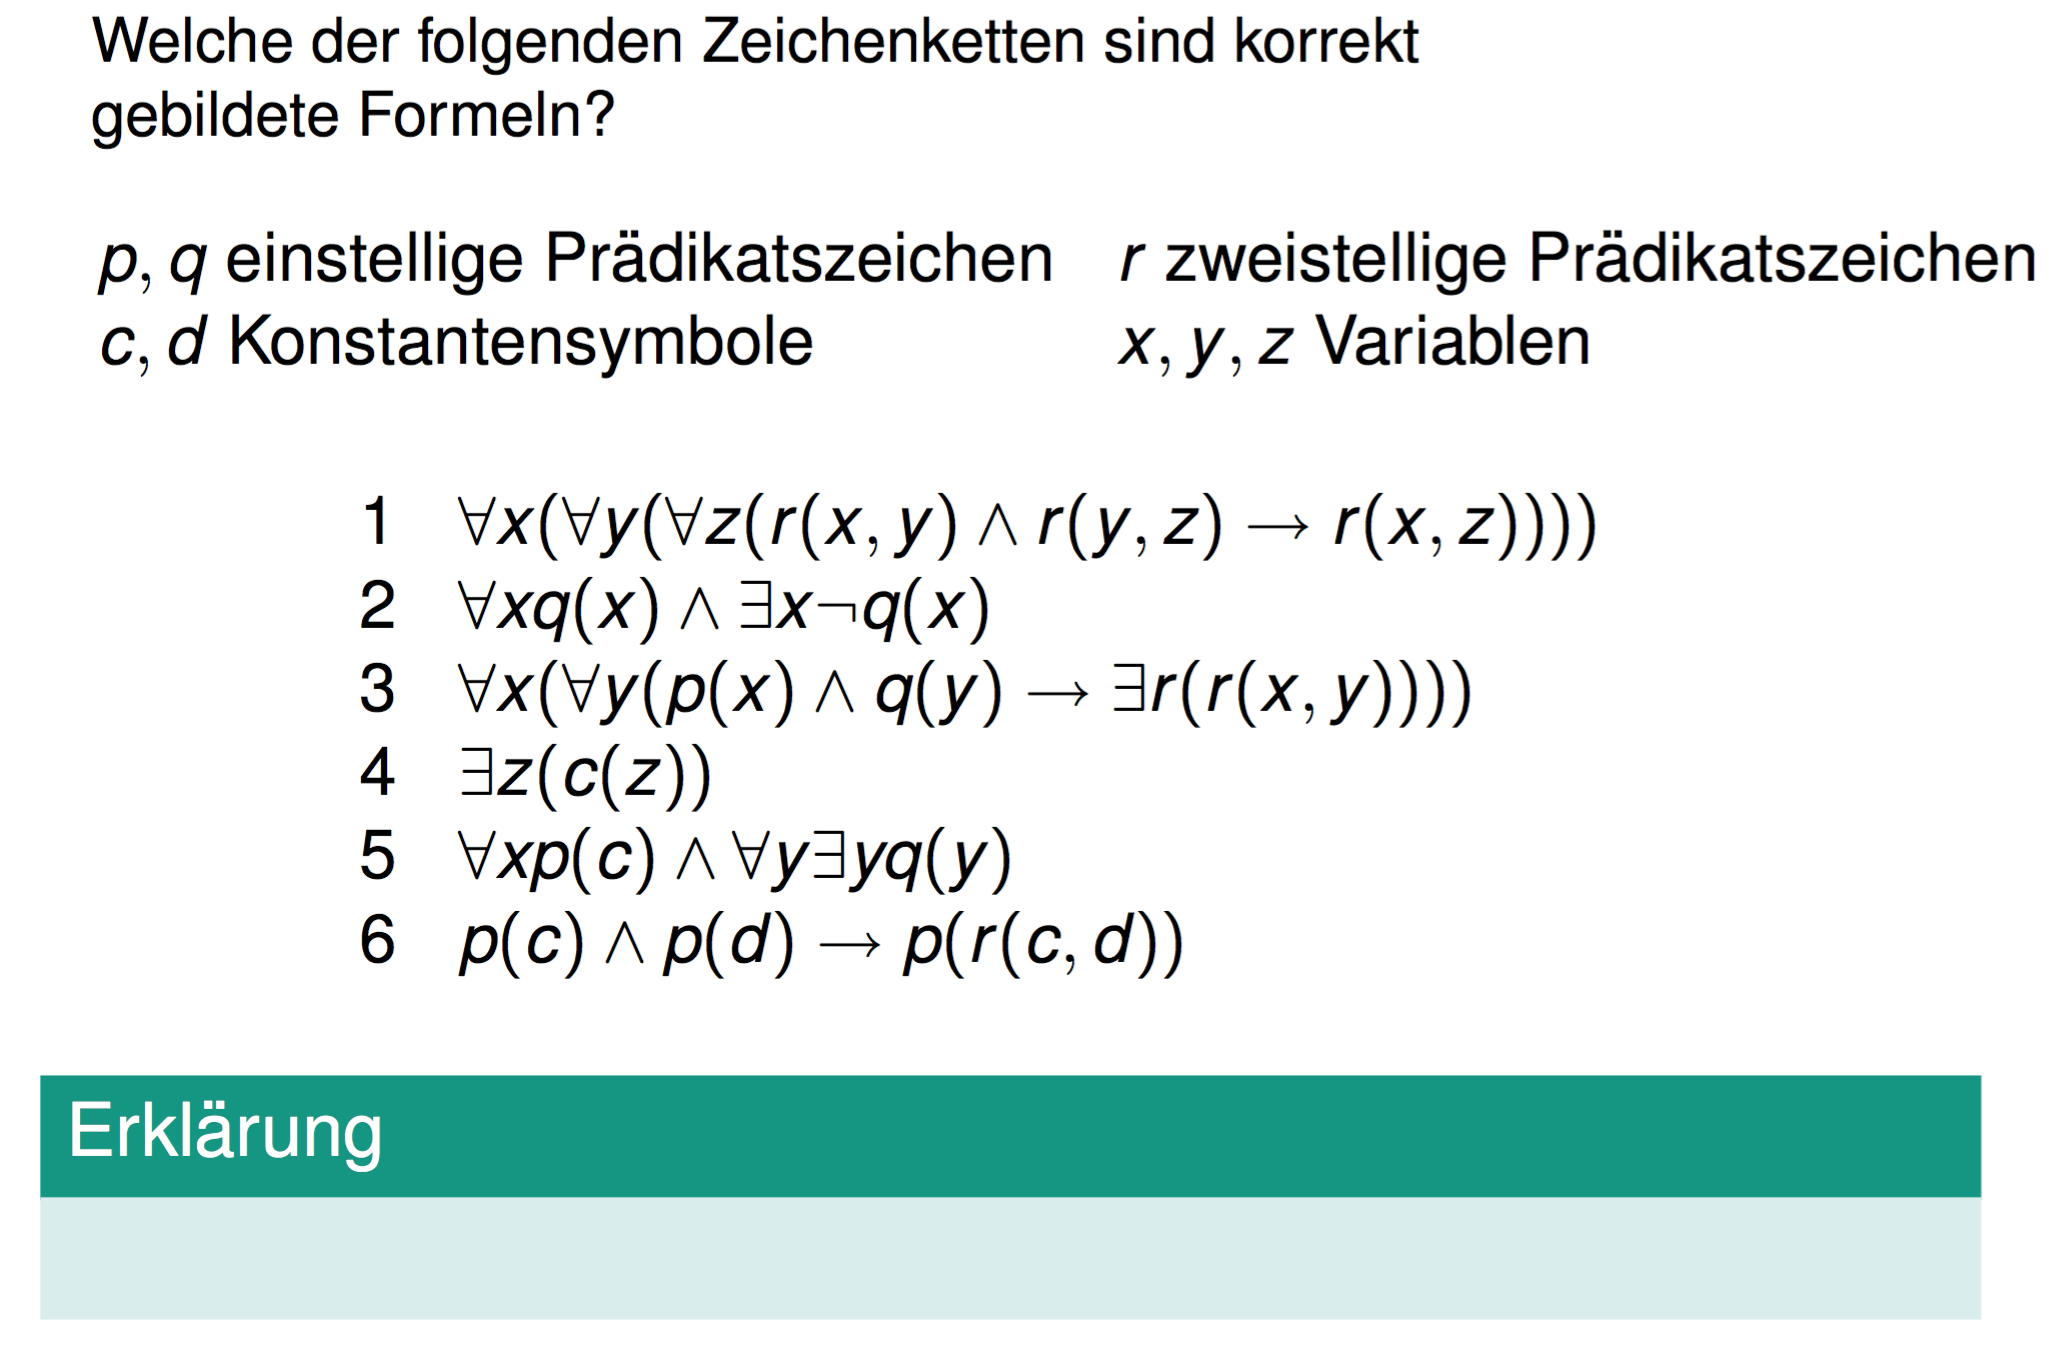
\includegraphics[scale=0.2]{q1.png}}
	\only<2|handout:2>{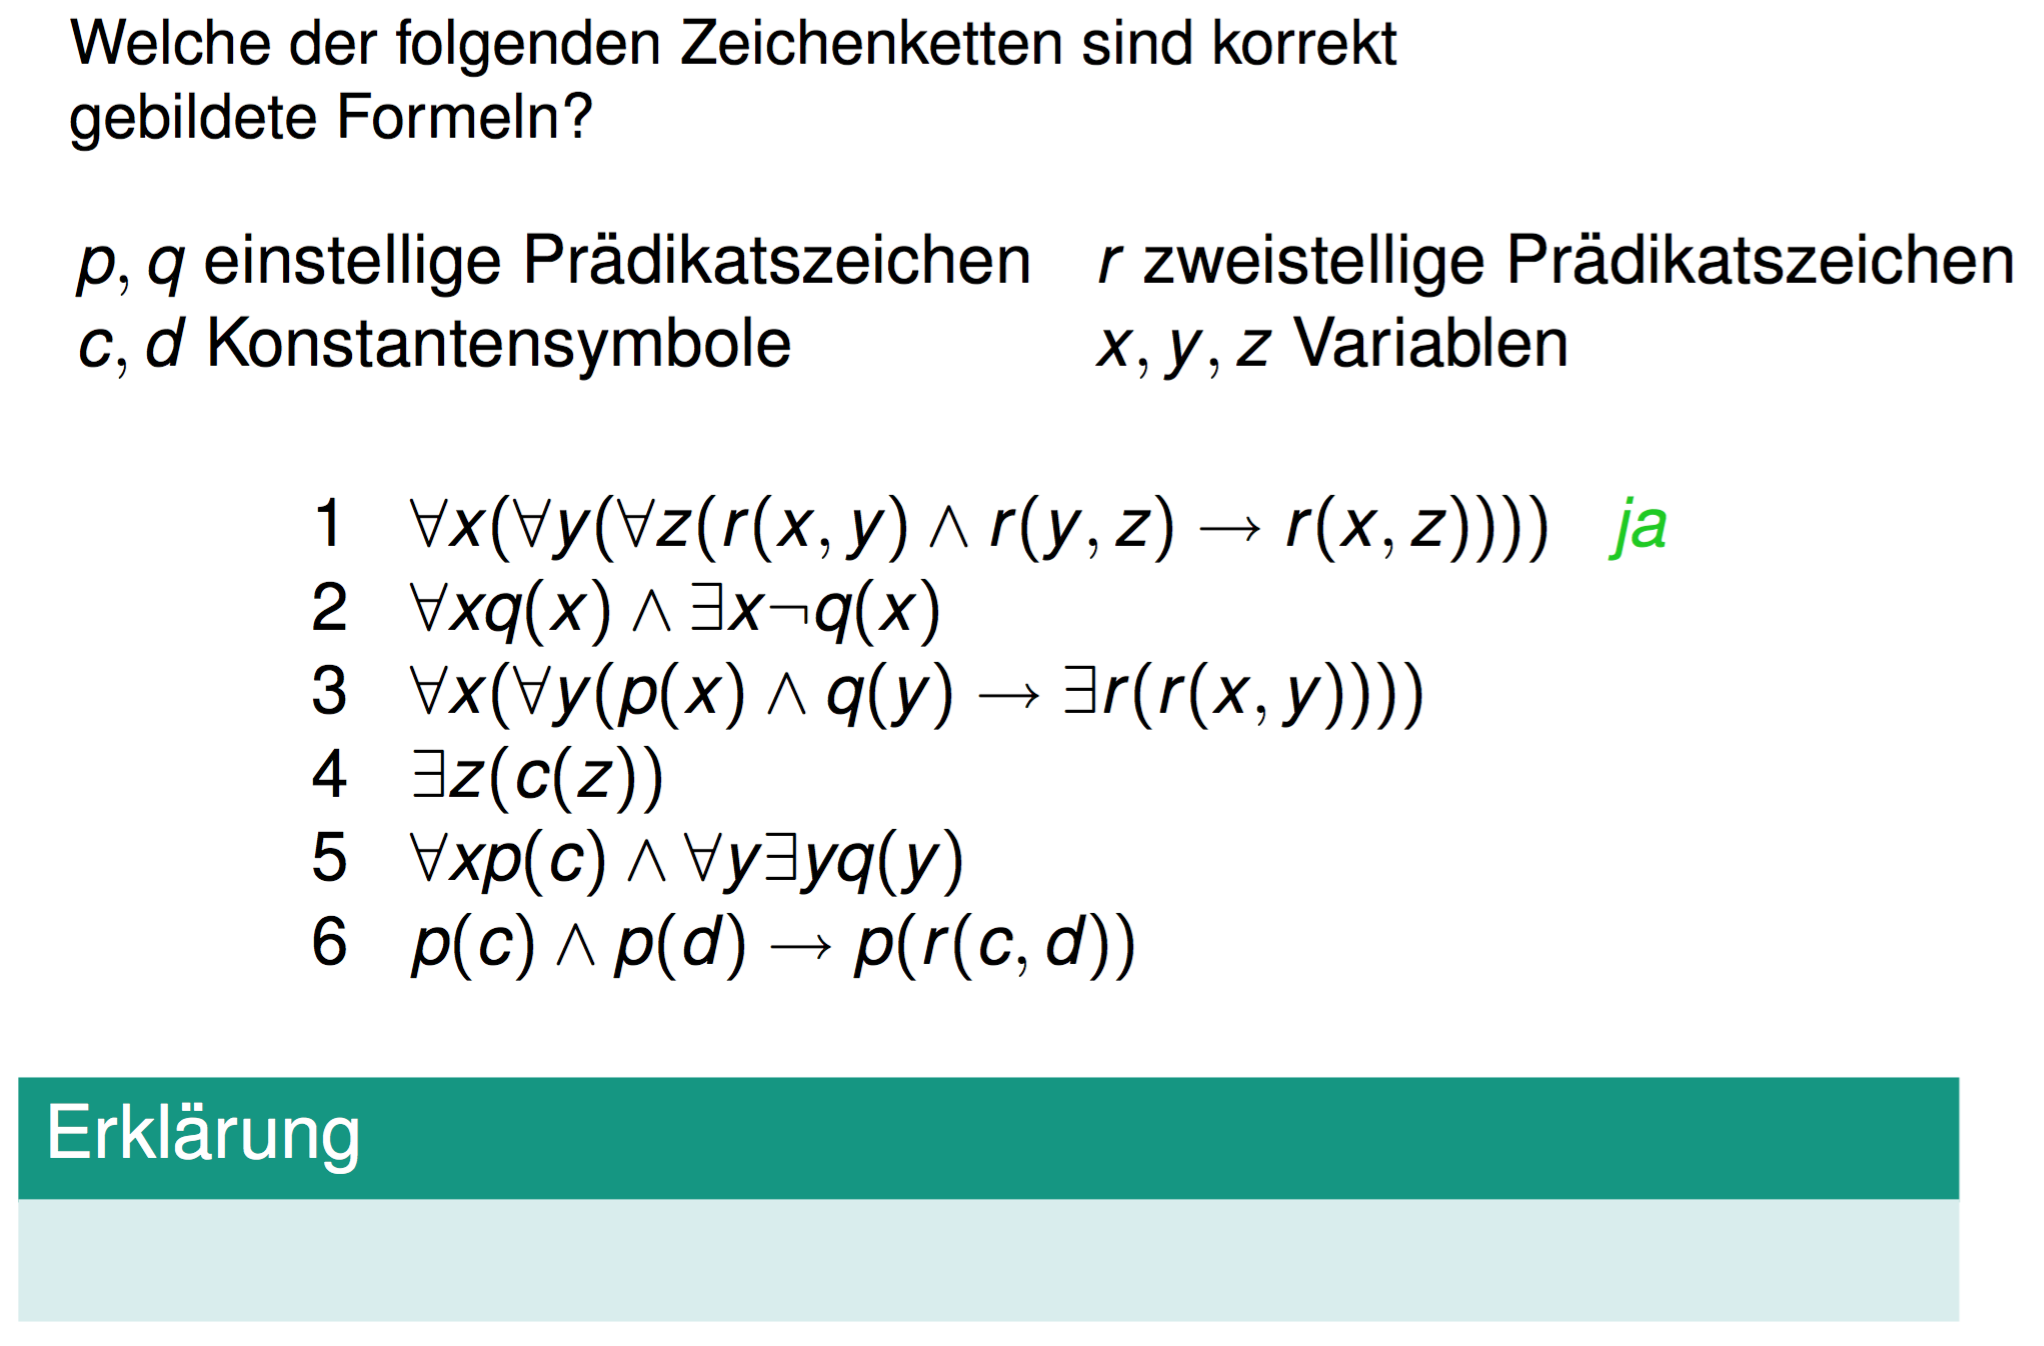
\includegraphics[scale=0.2]{q2.png}} 
	\only<3|handout:3>{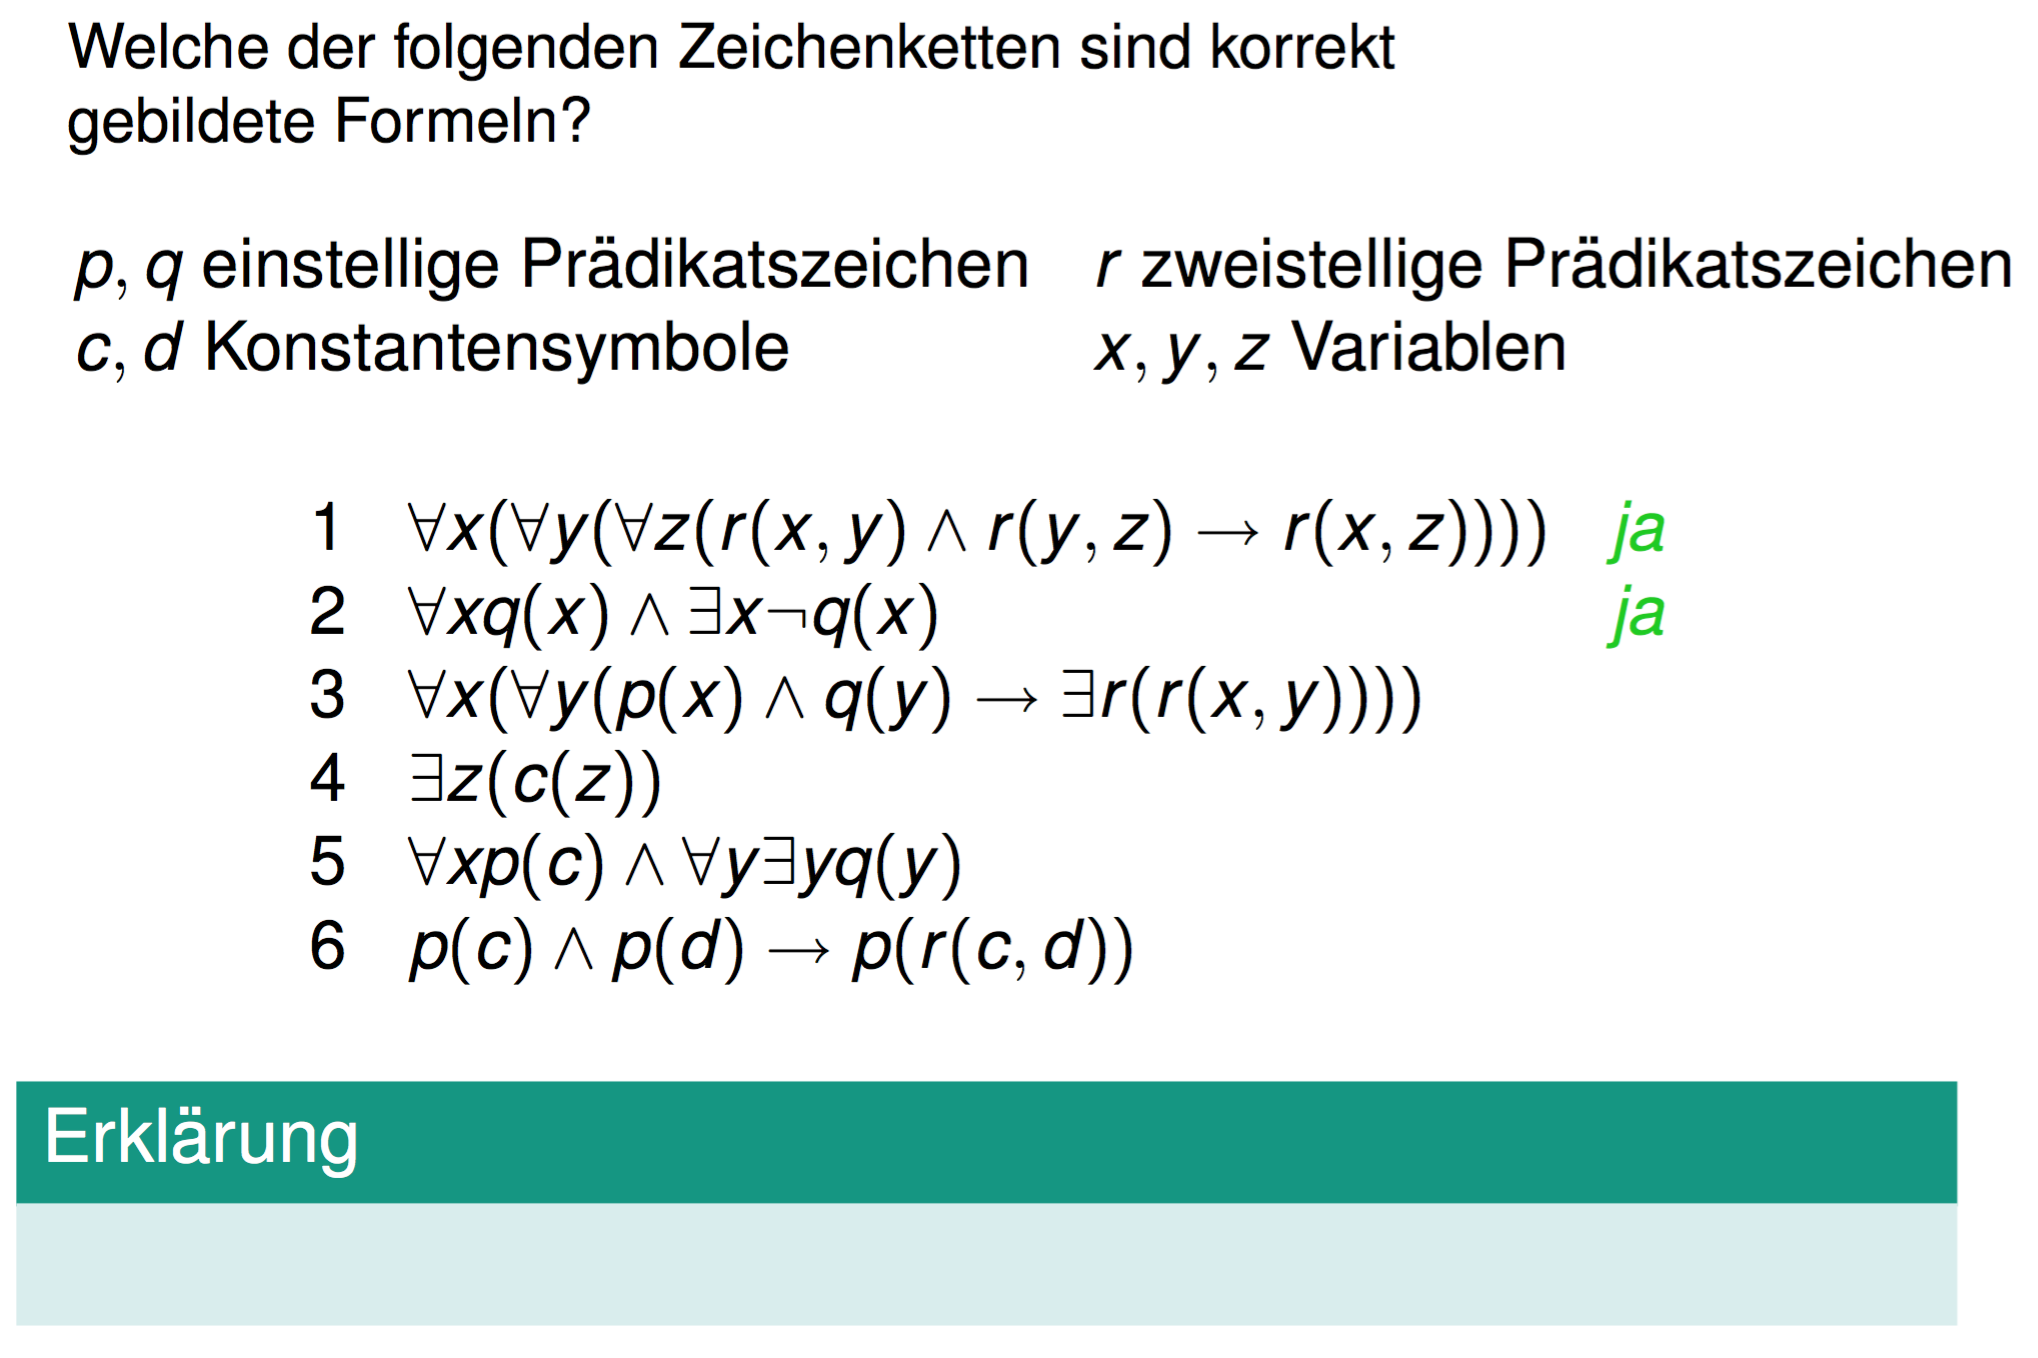
\includegraphics[scale=0.2]{q3.png}}
	\only<4|handout:4>{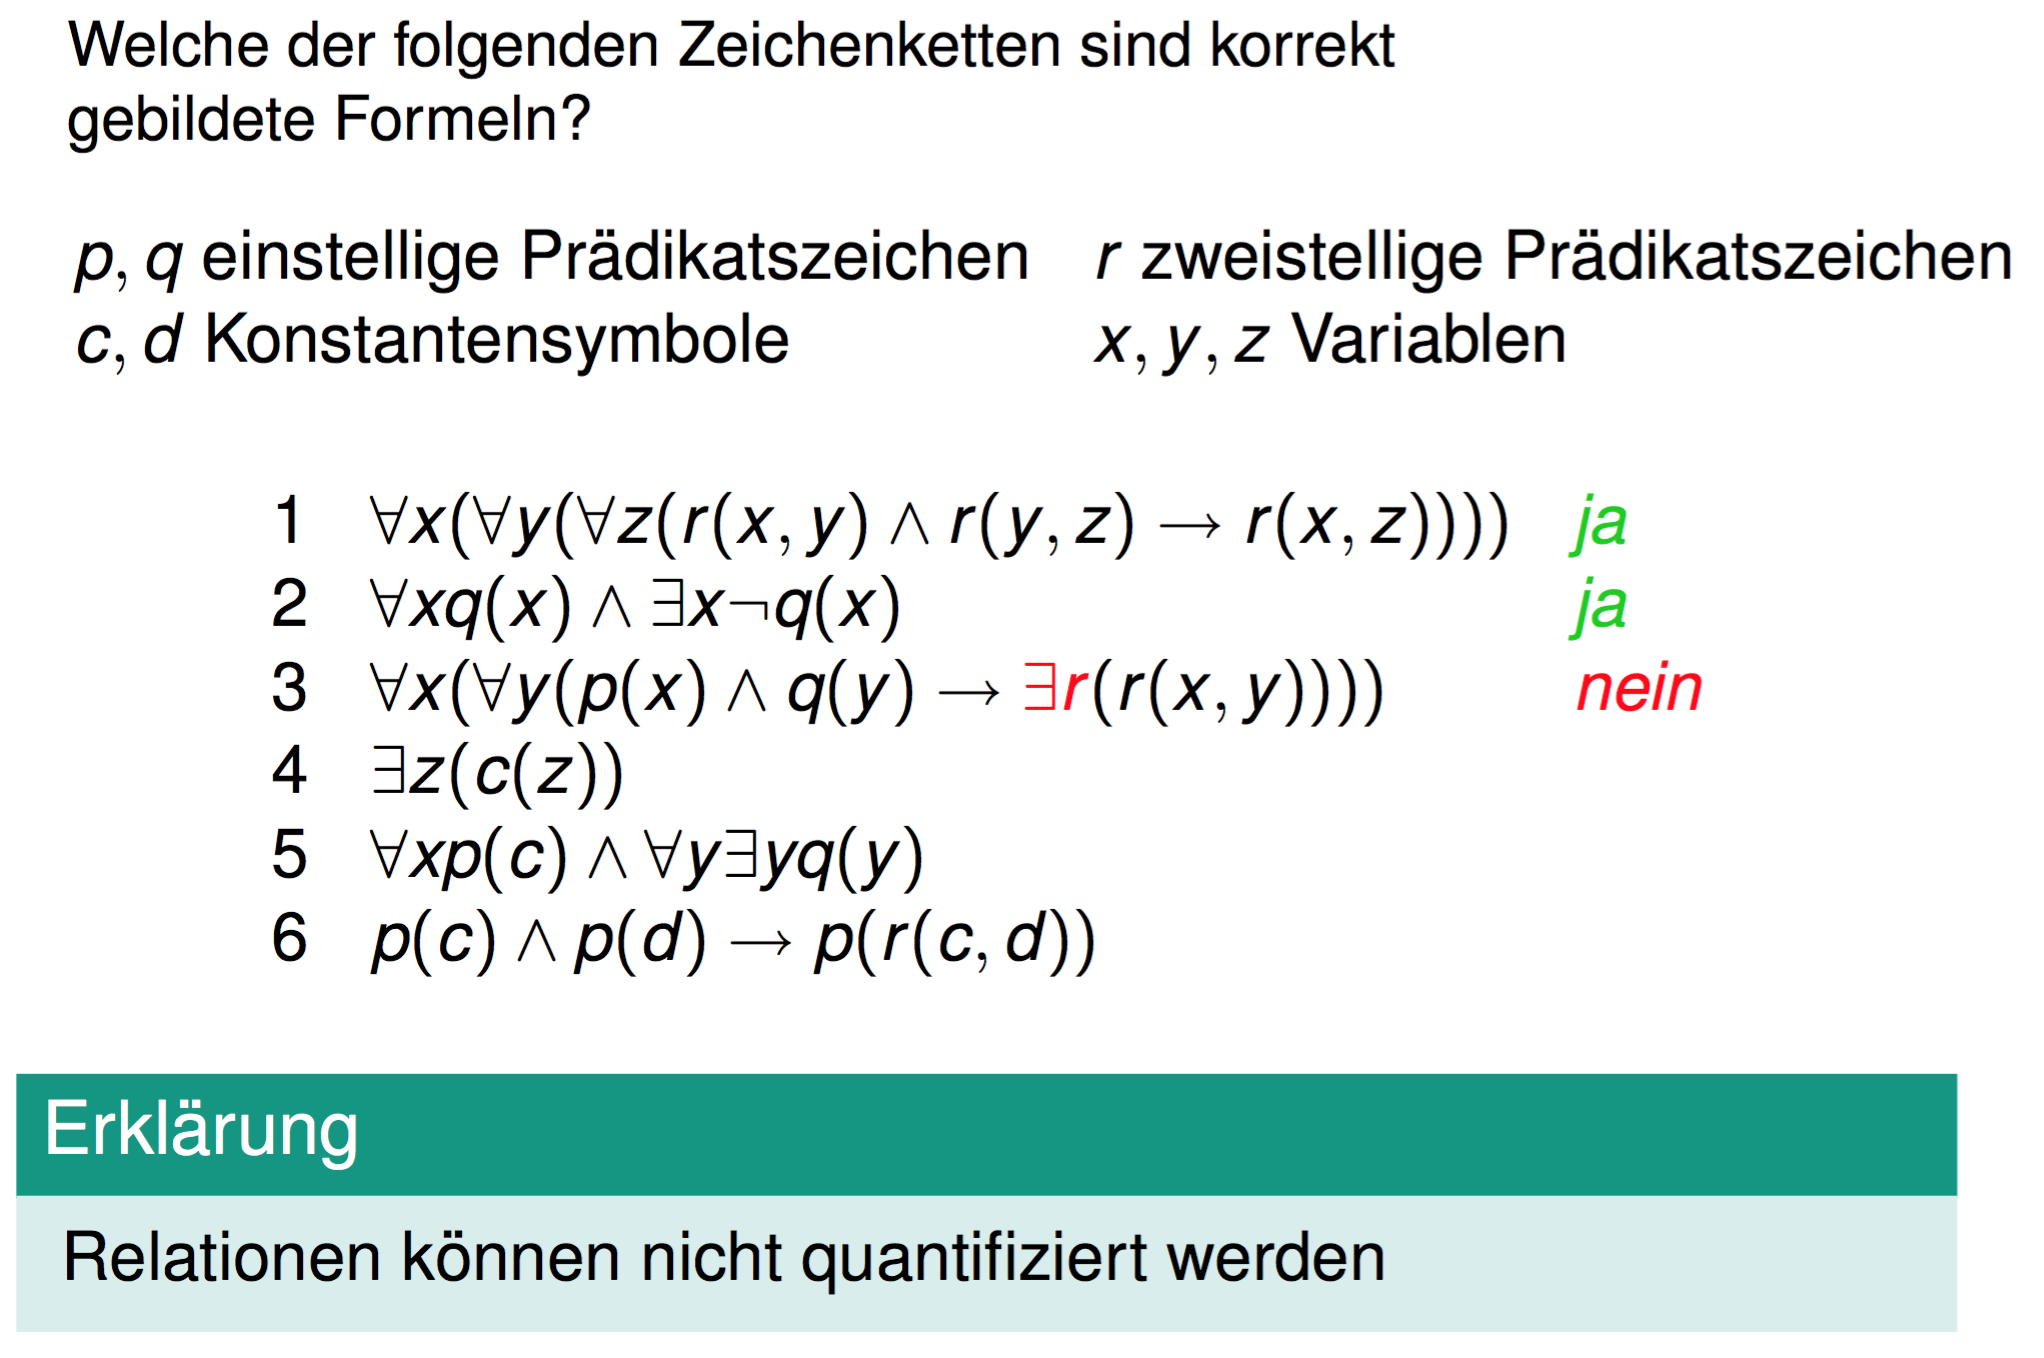
\includegraphics[scale=0.2]{q4.png}}
	\only<5|handout:5>{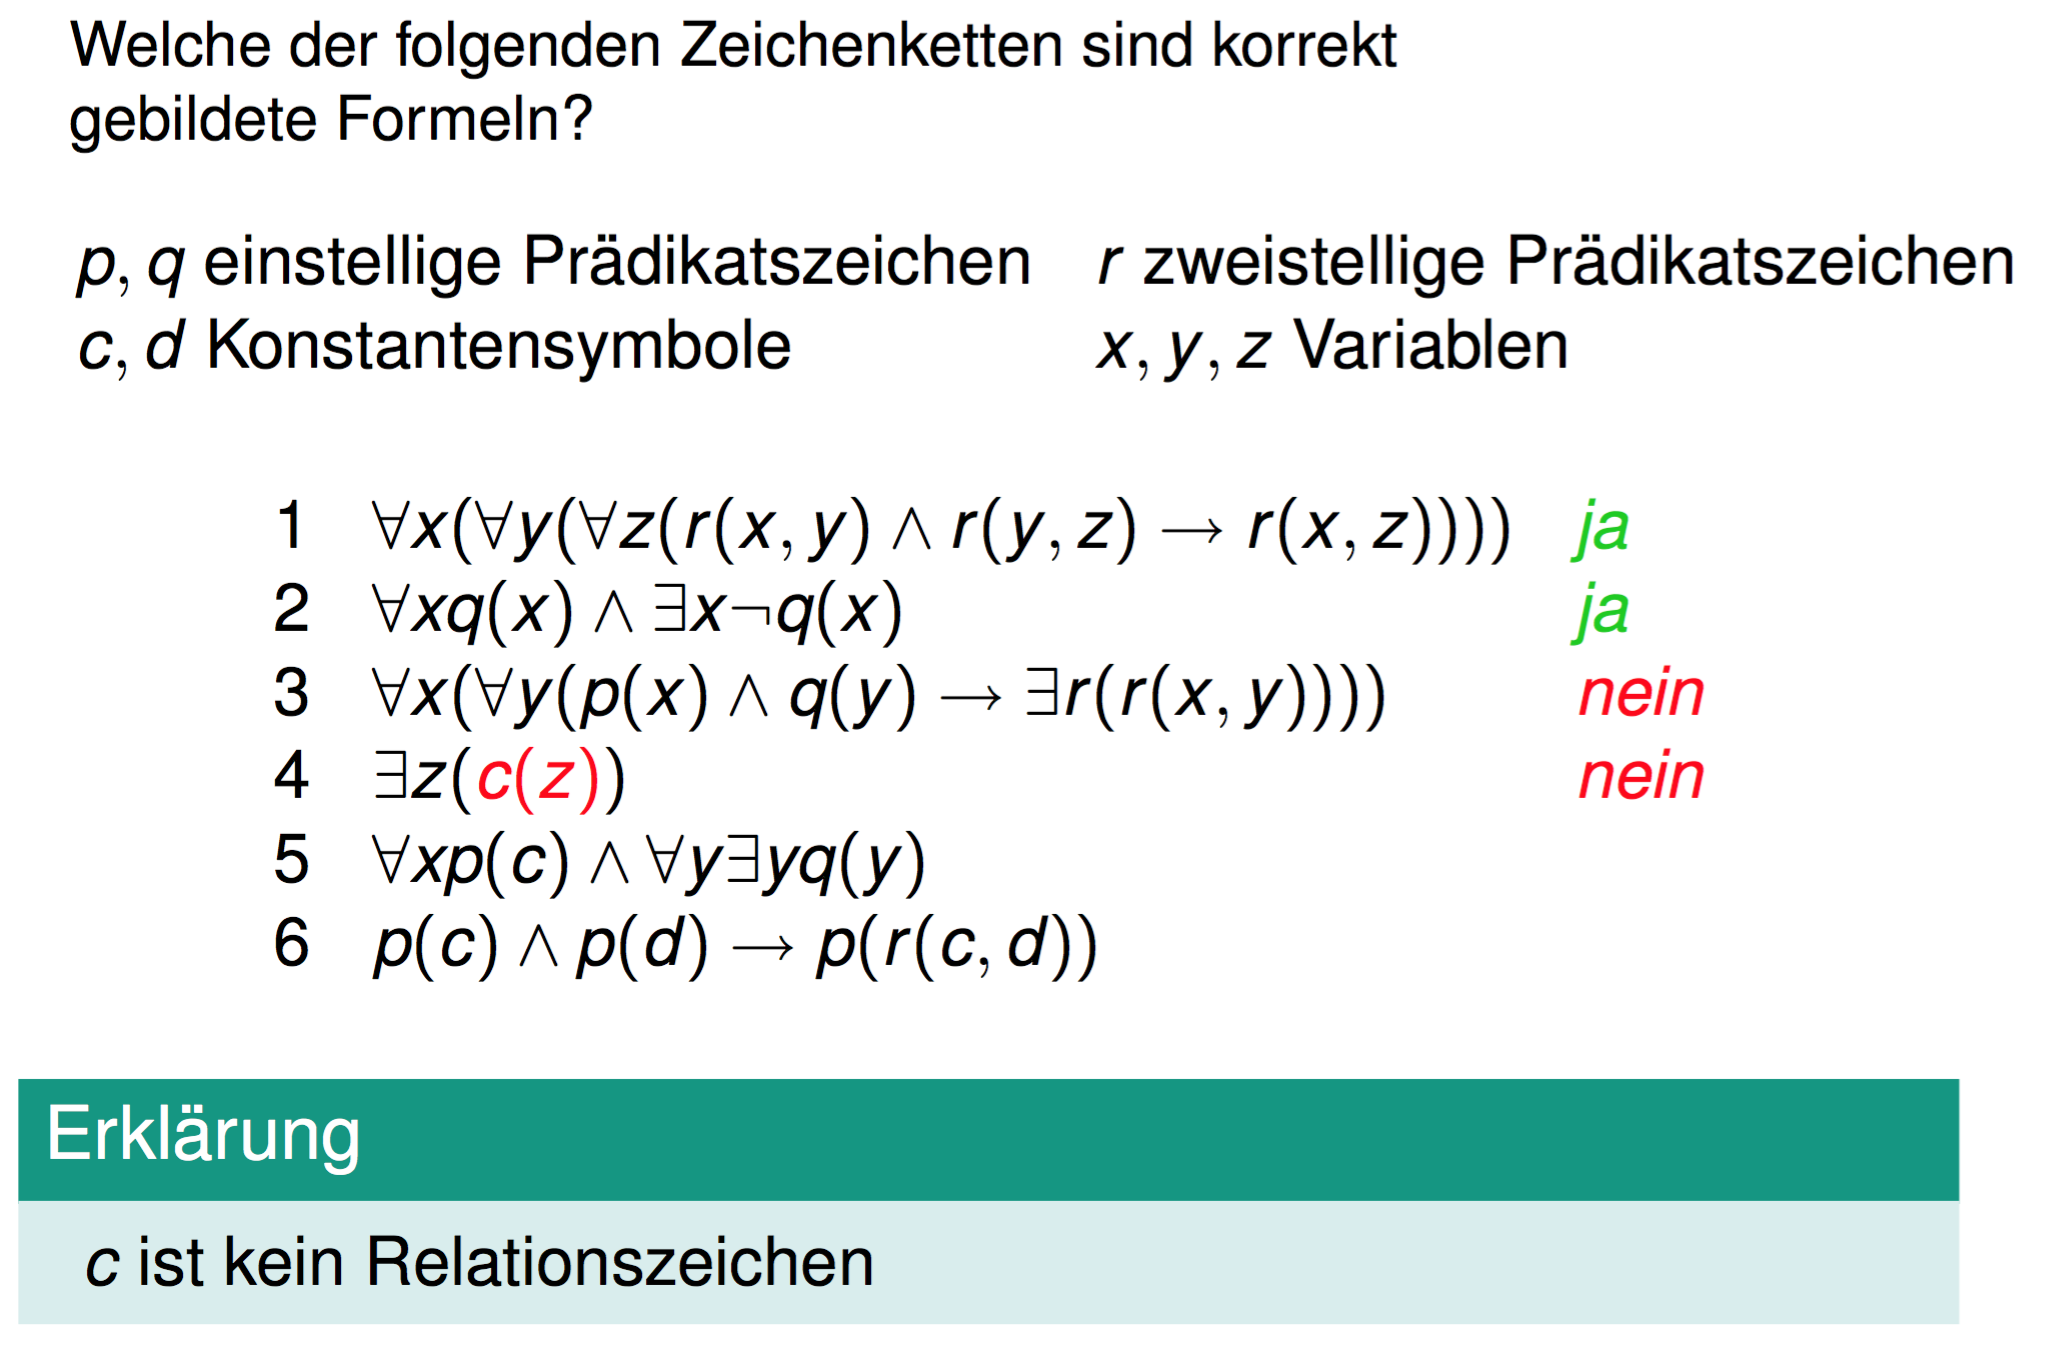
\includegraphics[scale=0.2]{q5.png}}
	\only<6|handout:6>{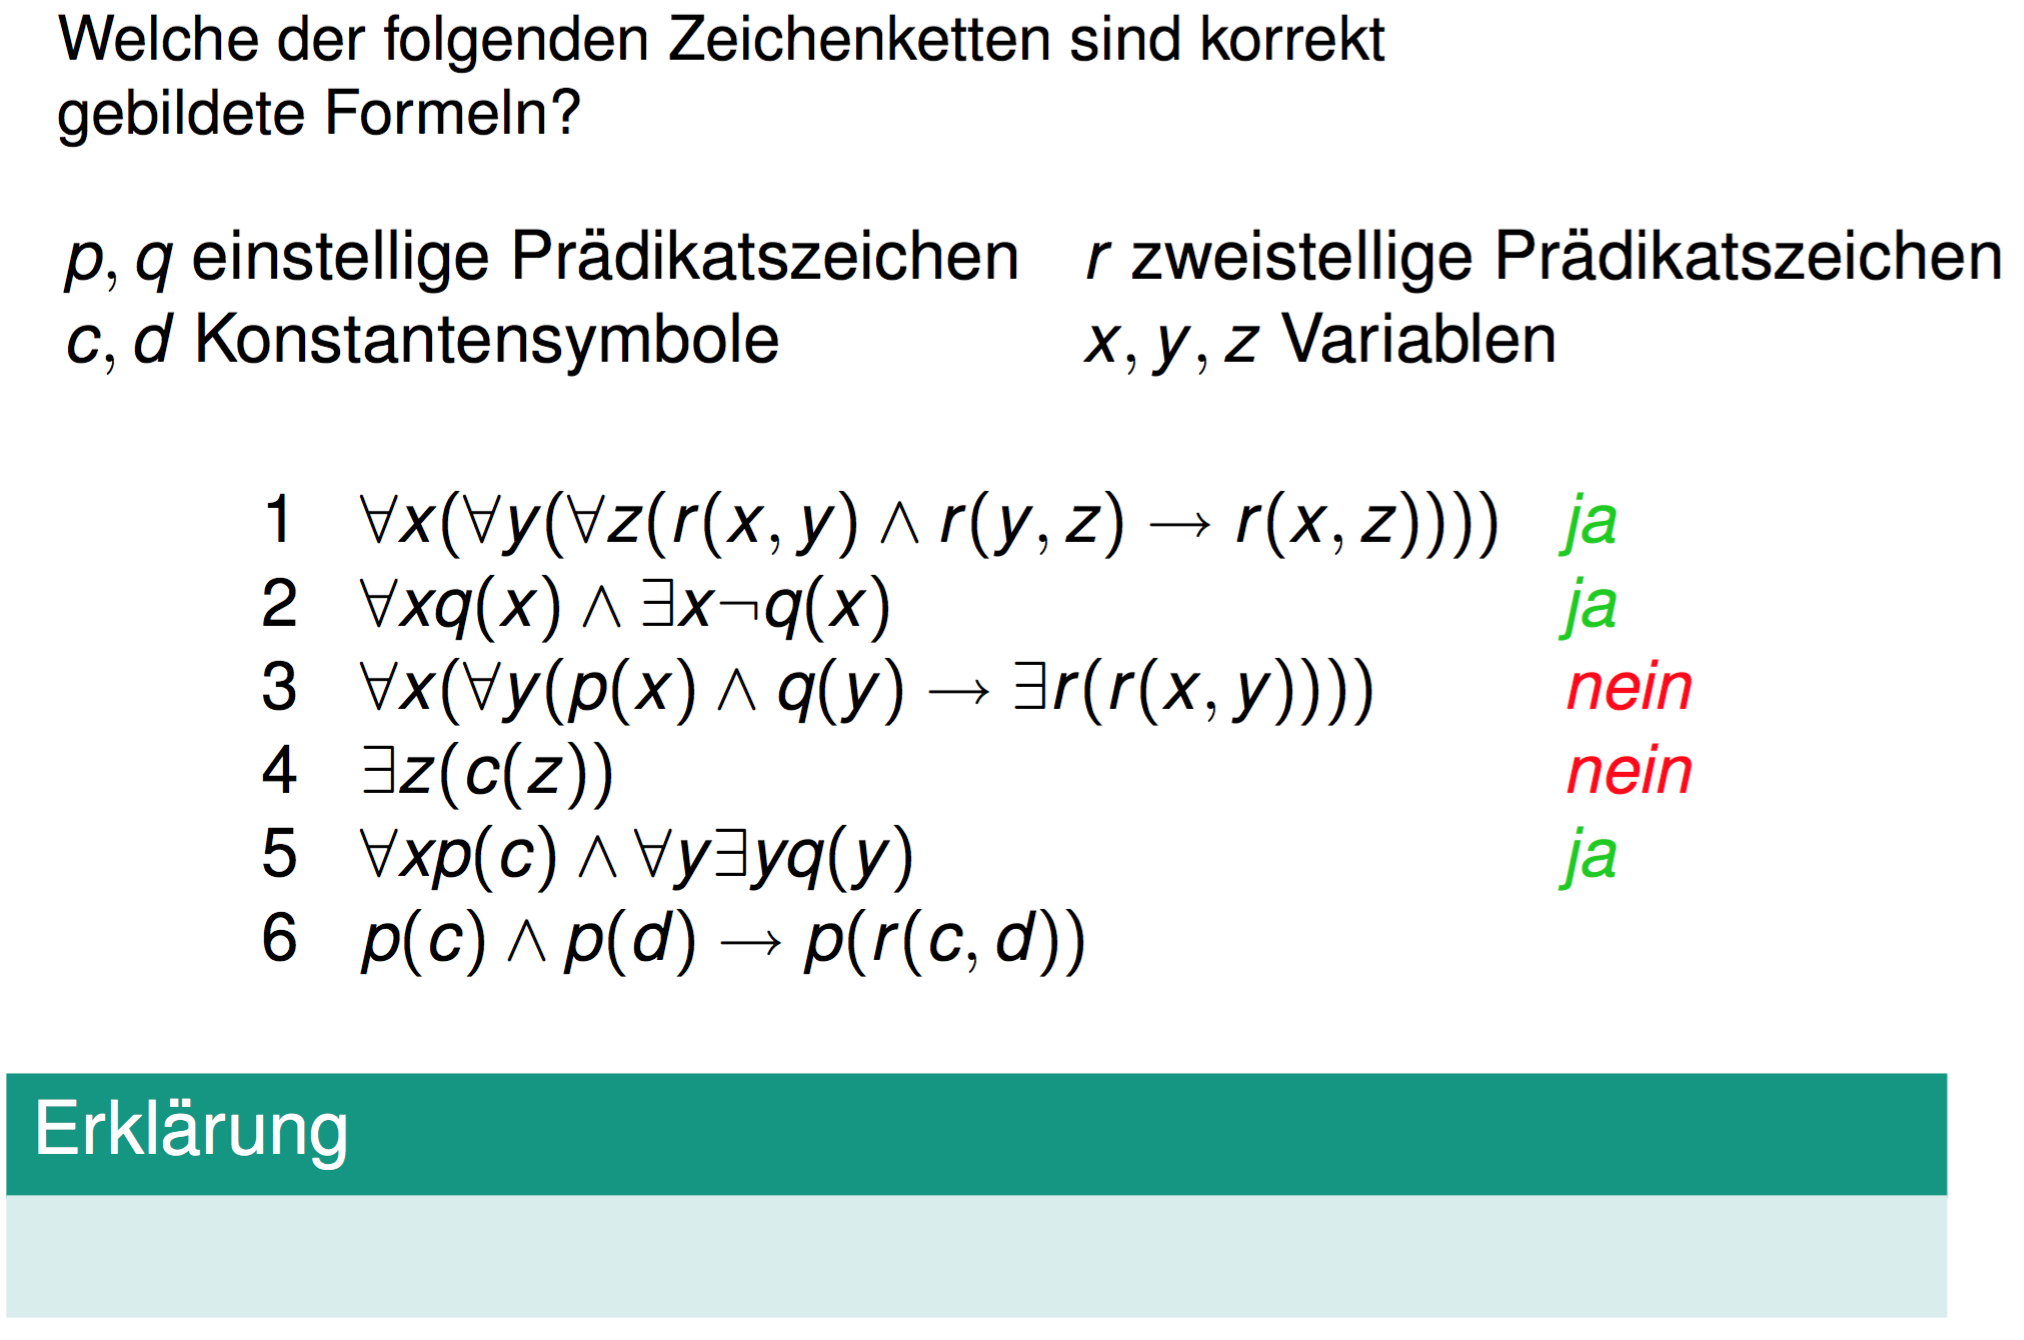
\includegraphics[scale=0.2]{q6.png}}
	\only<7|handout:7>{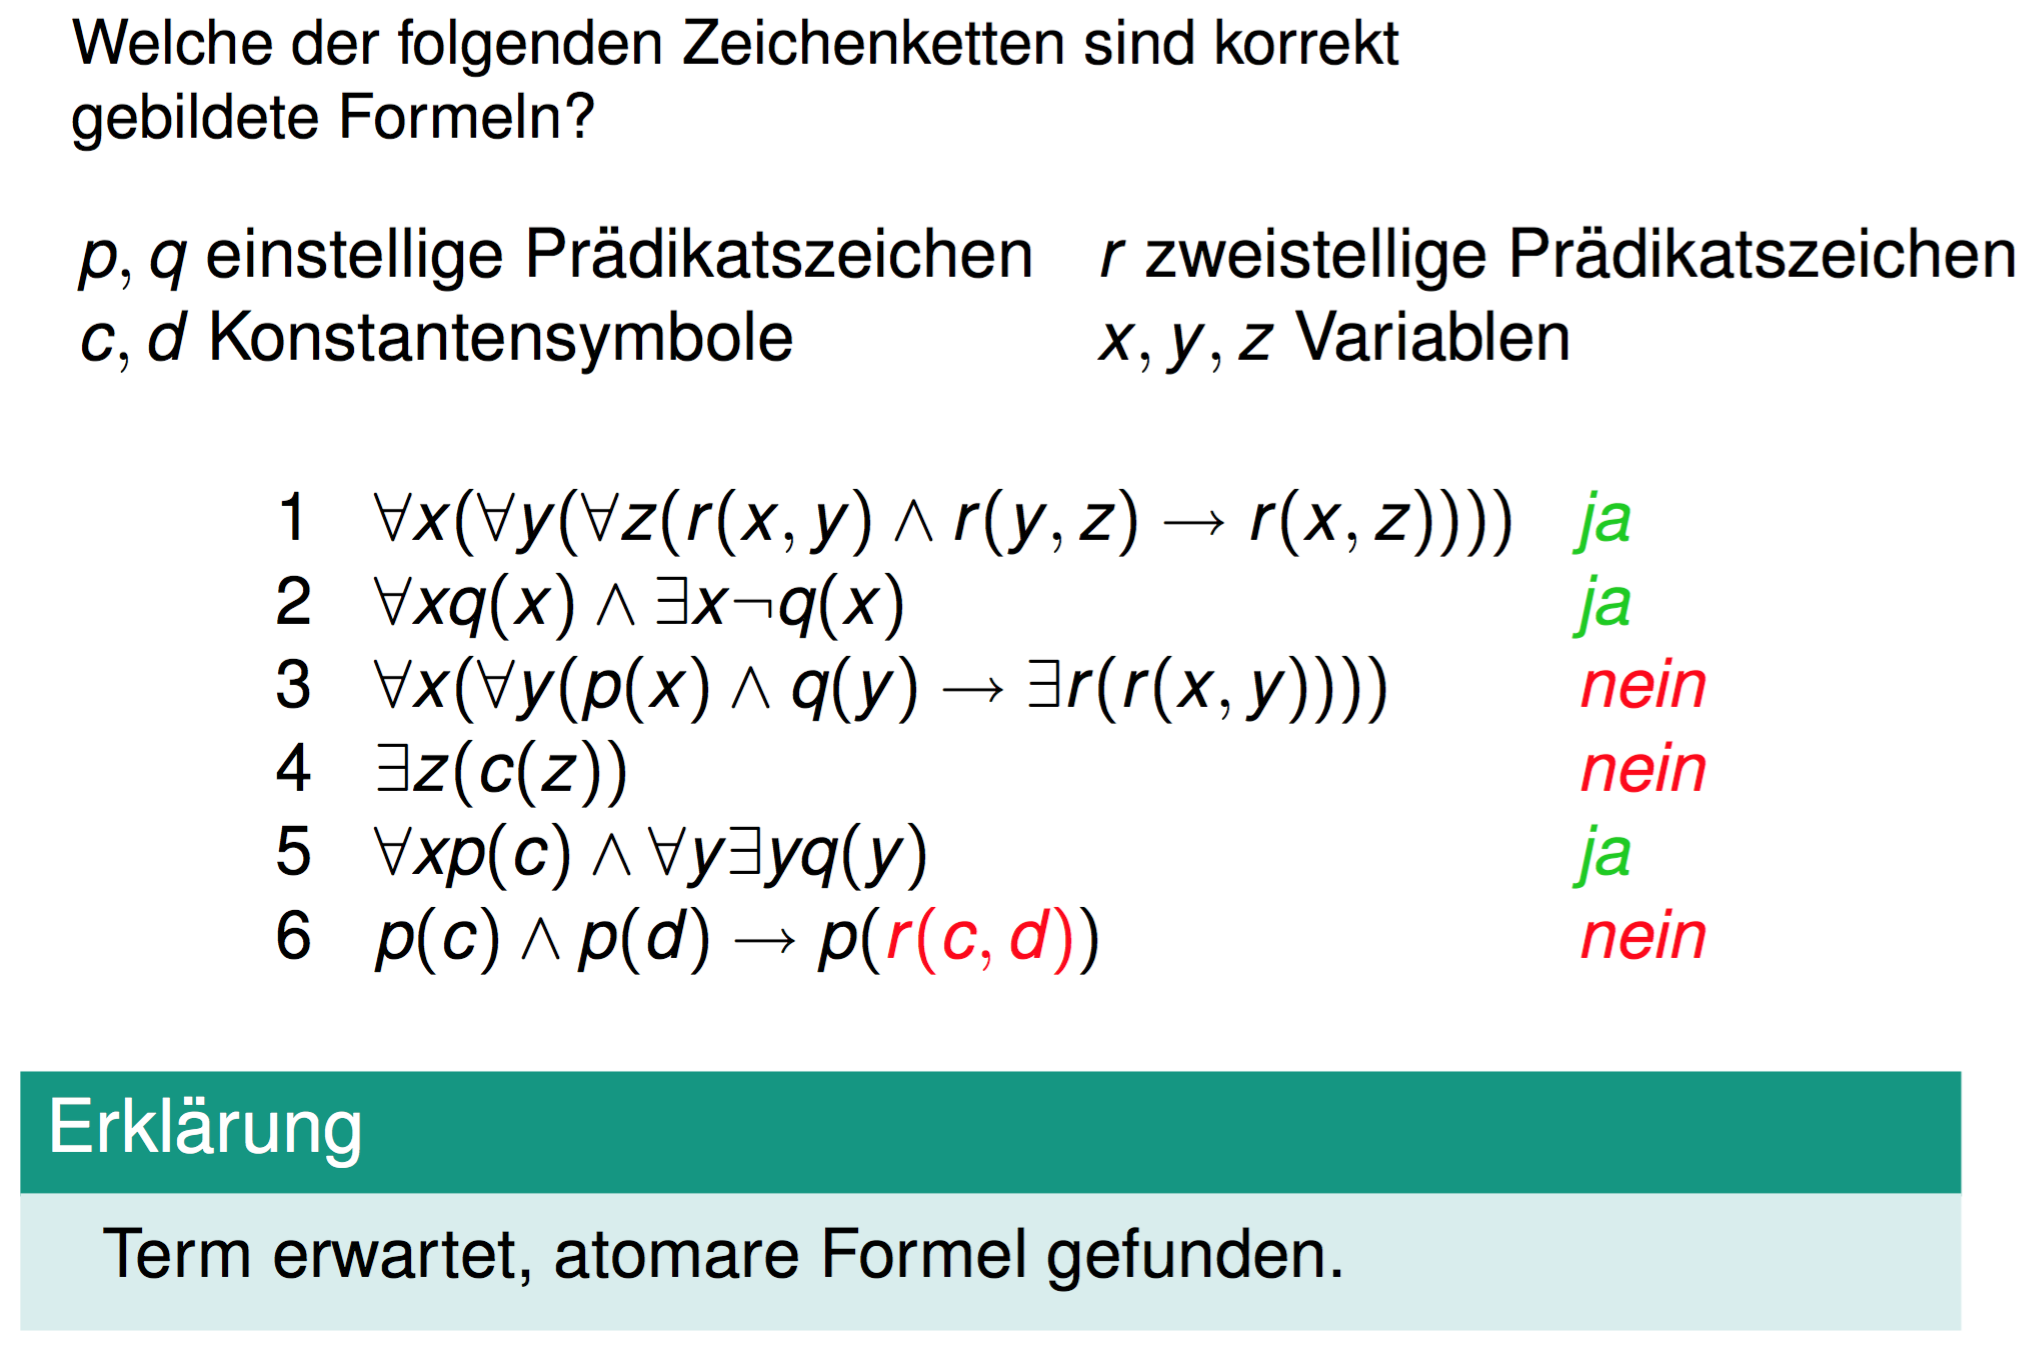
\includegraphics[scale=0.2]{q7.png}}
	\hspace{2em}
\end{figure} 
\end{frame}

\begin{frame}{Aufgabe 2 (WS 15/16, Blatt 7)}
	\begin{block}{Aufgabe}
		Formuliert die folgenden Aussagen als Formeln in Prädikatenlogik:
		\begin{enumerate}
			\item Nicht alle Vögel können fliegen.
			\item Wenn es irgendjemand kann, dann kann es Donald Ervin Knuth.
			\item John liebt jeden, der sich nicht selbst liebt.
		\end{enumerate}
	\end{block}
	
	\visible<2-|handout:2>{
		\begin{block}{Lösung}
			\begin{enumerate}
				\item \qquad $\plexist \plx {\plka \plfoo{Vogel}{\plka \plx \plkz} \aland \alnot \plfoo{flugfähig}{\plka \plx \plkz} \plkz}$
				\visible<3-|handout:2>{
					\item \qquad $
					\plexist \plx {\plka \plfoo{kann\_es}{\plka \plx \plkz} \plkz}
					\alimpl
					\plfoo{kann\_es}{\plka \plfoo{knuth} \plkz}
					$
				}
				\visible<4-|handout:2>{
					\item \qquad $
					\plall \plx {\plka \alnot \plfoo{liebt}{\plka \plx \plcomma \plx \plkz} \alimpl \plfoo{liebt}{\plka \plfoo{John} \plcomma \plx \plkz} \plkz}
					$
				}
			\end{enumerate}
		\end{block}
	}
\end{frame}

\begin{frame}{Freie und gebundene Variablenvorkommen}
	\textbf{Vorkommen} einer Variable in einer PL-Formel: \\
	$G = \plall \word{x\,R(\underline{x})}$ \Impl \word x kommt in $G$ vor. \\
	„Direkt hinter Quantoren“ zählt nicht! \\
	Bsp.: $F = \plall \word{x\,R(c)}$ \Impl \word x kommt \textbf{nicht} in $F$ vor! \\
	\medskip \pause
	
	\textbf{Freie Variablenvorkommen} \quad $\fv(F)$ \\
	Alle, die \emph{irgendwo} in $F$ vorkommen, ohne dass sie quantifiziert sind {\small ($=$ ein Quantor sie einführt)}. \\
	\medskip \pause
	
	\textbf{Gebundene Variablenvorkommen} \quad $\bv(F)$ \\
	Alle, die \emph{irgendwo} in $F$ vorkommen und dabei quantifziert sind. \\
	\medskip \pause
	
	Formel $F$ heißt \textbf{geschlossen} $:\!\!\Gdw \fv(F) = \emptyset$\\
	\medskip \pause
	 
	Beispiel: \\
	$\fv\left(\word{R(\underline{x},\underline{y},c)} \aland \plexist \word x\, \word x \pleq \underline{\word y}  \right) = \set{\word x, \word y}$ \\ 
	\pause
	$\bv\left(\word{R(x,y,c)} \aland \plexist \word x\, \underline{\word x} \pleq \word y \right) = \set{\word x}$
\end{frame}

\begin{frame}{Freie und gebundene Variablenvorkommen}
	\begin{equation*}
	F = \alnot \plexist \plx
	{\plka
		\plE{\plka \plx \plcomma \ply \plkz}
		\alor
		\alnot \plall \plz \plall \plx \plall \ply
		{\plka
			\plE{\plka \plx \plcomma \plz \plkz} \aland \plE{\plka \ply \plcomma \plz \plkz} \alimpl \plx \pleq \ply
			\plkz}
		\plkz}
	\end{equation*}
	
	\begin{block}{Aufgabe 1.1}
		Welche Variablenvorkommen sind frei ($\fv$) und welche gebunden ($\bv$)?\\
		Ist die Formel geschlossen?
	\end{block}

	\pause
	\begin{block}{Lösung}
		Nur die Variable $\fv(F) = \{\ply\}$ kommt frei in $F$ vor.\\
		Genau die Variablen $\bv(F) = \{\plx, \ply, \plz\}$ kommen gebunden in $F$ vor.\\
		Da $\fv(F) \neq \emptyset$, ist $F$ nicht geschlossen.
	\end{block}
	
\end{frame}
\begin{frame}{Substitutionen}
	Wollen \textbf{Variablen} (!) durch andere Terme ersetzen. \\
	\impl Eine Substitutionsabbildung $$\sigma_S \from \LFor \functionto \LFor, \; \text{längliche Definition s. VL}$$ wendet Ersetzungen aus $S$ auf eine Formel an. \\
	\medskip \pause
	
	Beispiel: \\
	$\sigma_{\set{\word x/\word y}}\left(\word x \pleq \word c\right) = \word y \pleq \word c$. \\
	$\sigma_{\set{\word x/\word{f(c)}}}\left(\word{R(x,y)} \aland \plexists \word y\,\word y \pleq \word x\right) = \word{R(\word{f(c)},y)} \aland \plexists \word y\,\word y \pleq \word{f(c)}$. \\
	\medskip \pause
	
	Mehrere auf einmal: \\
	$\sigma_{\set{\word x/\word y, \, \word y/\word x}}\left(\word x \pleq \word y\right) = \word y \pleq \word x$.
\end{frame}

\begin{frame}{Substitutionen}
	Ersetzt werden nur \textbf{freie Variablenvorkommen}!\\
	Gebundene Vorkommen, also Variablen im Wirkungsbereich eines Quantors, werden \textbf{nicht} ersetzt. \\
	\medskip \pause
	
	Beispiel: \\
	$\sigma_{\set{\word y/\word{f(c)}}}\left(\word{R(x,y)} \aland \plexists \word y\,\word y \pleq \word x\right) = \word{R(x,\word{f(c)})} \aland \plexists \word y\,\word y \pleq \word x$
	
\end{frame}

\begin{frame}{Substitutionen: Kollisionsfreiheit}
	Bei einer \textbf{kollisionsfreien} Substitution werden keine Variablen \enquote{aus Versehen} gebunden.\\[1em]
	Ersetzen wir eine freie Variable $\word x$ durch einen Term, in dem die Variable $\word y$ frei vorkommt, so darf sich $\word x$ nicht im Wirkungsbereich eines Quantors über $\word y$ befinden.
	
	\pause
	\begin{Beispiel}
		$F = \plall \plx \plka\plx \aland \ply\plkz$\\
		Kollisionsfrei: $\sigma_{\{\ply/\plz\}}$\\
		Nicht kollisionsfrei: $\sigma_{\{\ply/\plx\}}$
	\end{Beispiel}
\end{frame}

\begin{frame}{Substitutionen}
	\begin{equation*}
	F = \alnot \plexist \plx
	{\plka
		\plE{\plka \plx \plcomma \ply \plkz}
		\alor
		\alnot \plall \plz \plall \plx \plall \ply
		{\plka
			\plE{\plka \plx \plcomma \plz \plkz} \aland \plE{\plka \ply \plcomma \plz \plkz} \alimpl \plx \pleq \ply
			\plkz}
		\plkz}
	\end{equation*}
	
	\begin{block}{Aufgabe 1.2}
		Gebt eine Substitution $\sigma$ an, die \emph{nicht} kollisionsfrei für $F$ ist.\\[1em] \pause
		
		Die Substitution $\sigma_{\{\ply/\plx\}}$ leistet das Gewünschte.
	\end{block}
	
\end{frame}


\subsection{Prädikatenlogik: Semantik}

\begin{frame}{Interpretation}
	\begin{figure}[h!]
		\centering
		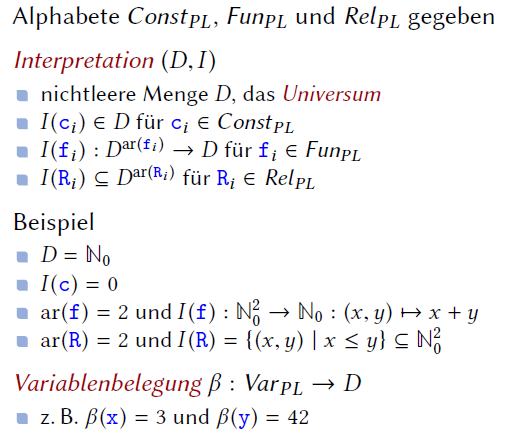
\includegraphics[scale=0.6]{int.png} \hspace{2em} 
	\end{figure} 
\end{frame}

\begin{frame}{Aufgabe 1 (WS 15/16, Blatt 7)}
	  \begin{equation*}
	\alnot \plexist \plx
	{\plka
		\plE{\plka \plx \plcomma \ply \plkz}
		\alor
		\alnot \plall \plz \plall \plx \plall \ply
		{\plka
			\plE{\plka \plx \plcomma \plz \plkz} \aland \plE{\plka \ply \plcomma \plz \plkz} \alimpl \plx \pleq \ply
			\plkz}
		\plkz}
	\end{equation*}\\[1em]
	
	\begin{block}{Aufgabe 1.3}
		Gebt eine Interpretation $(D_1, I_1)$ und eine Variablenbelegung $\beta_1$ so an, dass $val_{D_1, I_1, \beta_1}(F) = \W$ gilt.\\[0.5em]
		
		\visible<2-|handout:2>{Die Interpretation $(D_1, I_1) = (\{ 0, 1 \}, {<})$ und die Variablenbelegung $\beta_1 \colon \VPL \functionto D$, $v \mapsto 0$, leisten das Gewünschte.}
	\end{block}

	\begin{block}{Aufgabe 1.4}
		Gebt eine Interpretation $(D_2, I_2)$ und eine Variablenbelegung $\beta_2$ so an, dass $val_{D_2, I_2, \beta_2}(F) = \F$ gilt.\\[0.5em]
		
		\visible<3-|handout:2>{Die Interpretation $(D_2, I_2) = (\{ 0, 1 \}, {<})$ und die Variablenbelegung $\beta_2 \colon \VPL \functionto D$, $v \mapsto 1$, leisten das Gewünschte.}
	\end{block}
\end{frame}


%%%%%%%%%% %%%%%%%%%%
\section{}
\questionframe
\lastframe
\mode<handout>{\slideThanks}
\end{document}